% Desde docs/latex: latexmk -pdf -interaction=nonstopmode -halt-on-error -outdir=build report.tex
\documentclass[12pt,a4paper]{article}
\usepackage[spanish,es-nodecimaldot]{babel}
\usepackage[utf8]{inputenc}
\usepackage[T1]{fontenc}
\usepackage{lmodern}
\usepackage{amsmath,amssymb,graphicx,geometry,booktabs,tabularx,array,longtable}
\usepackage{fancyhdr,caption,setspace,microtype,xcolor,colortbl,enumitem,titlesec}
\usepackage{tikz}
\usetikzlibrary{calc,arrows.meta,positioning}
\usepackage[authoryear,round]{natbib}
\usepackage{xurl,float}
\usepackage[hidelinks]{hyperref}
\definecolor{NCPrimary}{HTML}{123D3B}
\definecolor{NCAction}{HTML}{164F46}
\definecolor{NCMint}{HTML}{BEE0D3}
\definecolor{NCAccent}{HTML}{E4B85A}
\definecolor{NCBackground}{HTML}{F4F6F5}
\definecolor{NCSurfaceMuted}{HTML}{E8EFEB}
\definecolor{NCText}{HTML}{25343B}
\definecolor{NCTextSecondary}{HTML}{52655D}
\definecolor{NCBorder}{HTML}{DCE4E0}
\geometry{margin=2.35cm}
\setstretch{1.12}
\setlength{\parindent}{0pt}
\setlength{\parskip}{5pt}
\setlength{\headheight}{25pt}
\setlength{\emergencystretch}{3em}
\color{NCText}
\pagestyle{fancy}\fancyhf{}
\lhead{\color{NCPrimary}\small FHCP Challenge}
\rhead{\color{NCTextSecondary}\small Informe técnico y comparativo}
\cfoot{\color{NCPrimary}\thepage}
\renewcommand{\headrulewidth}{0.8pt}
\renewcommand{\headrule}{\hbox to\headwidth{\color{NCAccent}\leaders\hrule height \headrulewidth\hfill}}
\titleformat{\section}{\Large\bfseries\color{NCPrimary}}{\thesection}{0.65em}{}
\titleformat{\subsection}{\large\bfseries\color{NCAction}}{\thesubsection}{0.65em}{}
\titlespacing*{\section}{0pt}{1.1em}{0.5em}
\titlespacing*{\subsection}{0pt}{0.7em}{0.3em}
\captionsetup{font=small,labelfont=bf,skip=6pt}
\setlist{nosep,leftmargin=1.4em,topsep=4pt}
\arrayrulecolor{NCBorder}
\setcounter{tocdepth}{1}
\newcolumntype{Y}{>{\raggedright\arraybackslash}X}
\newcommand{\pagina}[1]{\clearpage\section{#1}}
\newcommand{\code}[1]{{\small\path{#1}}}
\newcommand{\TotalAttempts}{8\,806}
\newcommand{\TotalSuccesses}{345}
\newcommand{\SolvedGraphs}{15}
\newcommand{\TotalErrors}{12}
\newcommand{\TotalExhausted}{8\,449}
\newcommand{\PendingAttempts}{51\,254}
\newcommand{\SuccessRate}{3.92}
\newcommand{\CompleteGraphs}{144}
\newcommand{\StartedGraphs}{149}
\newcommand{\PartialGraphs}{5}
\newcommand{\UnstartedGraphs}{852}
\newcommand{\AttemptsPerFamily}{1\,440}

\newcommand{\RepairAttempts}{2\,976}
\newcommand{\RepairSuccesses}{11}
\newcommand{\RepairErrors}{4}
\newcommand{\RepairExhausted}{2\,961}
\newcommand{\RepairSolved}{5}
\newcommand{\RepairComplete}{48}
\newcommand{\RepairPartial}{4}
\newcommand{\RepairStarted}{52}
\newcommand{\RepairUnstarted}{13}
\newcommand{\RepairOmitted}{924}
\newcommand{\RepairCoverage}{76.31}
\newcommand{\RepairBalancedDenominator}{480}
\newcommand{\RepairSessionHours}{6.37}
\newcommand{\UnionCertifiedGraphs}{22}
\newcommand{\PriorAttempts}{118}
\newcommand{\PriorErrors}{4}
\newcommand{\PriorSuccesses}{2}

\hypersetup{pdftitle={Metaheurísticas para ciclos hamiltonianos: evaluación FHCP},pdfauthor={Zapata Aguilar; Euresti; Zúñiga Zavala; Zúñiga de León; Vazquez Leonel},pdfsubject={Fundamentos de Inteligencia Artificial, Universidad Politécnica de Victoria}}
\AddToHook{shipout/background}{\ifnum\value{page}>1\begin{tikzpicture}[remember picture,overlay]\fill[NCAction] (current page.south west) rectangle ([xshift=.35cm]current page.north west);\end{tikzpicture}\fi}
\begin{document}
\begin{titlepage}\thispagestyle{empty}
\begin{tikzpicture}[remember picture,overlay]
\fill[NCBackground] (current page.south west) rectangle (current page.north east);
\begin{scope}[transform canvas={rotate around={35:($(current page.north west)+(-1,-2)$)}}]
\shade[rounded corners=18pt,left color=NCAccent,right color=NCMint] ($(current page.north west)+(-1,-2)$) rectangle ++(13,1.3);
\end{scope}
\begin{scope}[transform canvas={rotate around={35:($(current page.north east)+(-9,-1)$)}}]
\shade[rounded corners=15pt,left color=NCAction,right color=NCMint] ($(current page.north east)+(-9,-1)$) rectangle ++(13,.8);
\end{scope}
\fill[NCPrimary] (current page.south west) rectangle ([yshift=1.1cm]current page.south east);
\end{tikzpicture}
\vspace*{3.1cm}
{\color{NCPrimary}\Large\bfseries Universidad Politécnica de Victoria\par}
\vspace{.3cm}
{\color{NCTextSecondary}\normalsize Ingeniería en Tecnologías de la Información\\e Innovación Digital\par}
\vspace{1.0cm}
{\color{NCAction}\small\bfseries FUNDAMENTOS DE INTELIGENCIA ARTIFICIAL\par}
\vspace{.35cm}
{\color{NCPrimary}\fontsize{29}{35}\selectfont\bfseries Metaheurísticas para\\ciclos hamiltonianos\par}
\vspace{.35cm}
{\color{NCAction}\Large Evaluación técnica y comparativa\\sobre el FHCP Challenge Set\par}
\vspace{.5cm}
{\color{NCAccent}\rule{5cm}{2pt}\par}
\vspace{.45cm}
{\bfseries Profesor:} Dr. Said Polanco Martagón
\vspace{.7cm}

{\color{NCPrimary}\bfseries Integrantes}\par
\vspace{.15cm}
\begin{tabularx}{\linewidth}{@{}Yr@{}}
Diego Eduardo Zapata Aguilar & 2430053\\[4pt]
Cesar Euresti & 2430233\\[4pt]
Eder Omar Zúñiga Zavala & 2430206\\[4pt]
Elías de Jesús Zúñiga de León & 2430085\\[4pt]
Junior Arturo Vazquez Leonel & 2430319
\end{tabularx}
\vfill
{\color{NCTextSecondary}\small Fecha de entrega: 17 de noviembre de 2026\par}
\vspace{.5cm}
\end{titlepage}

\section*{Resumen}\addcontentsline{toc}{section}{Resumen}
Se implementaron seis metaheurísticas para buscar ciclos hamiltonianos en instancias del FHCP Challenge Set: algoritmo genético (GA), recocido simulado (SA), Ant System (AS, de la familia ACO), colonia artificial de abejas (ABC), evolución diferencial (DE) y optimización por enjambre de partículas (PSO). El problema se representó mediante permutaciones de vértices y un costo que cuenta las aristas ausentes, incluido el cierre de la ruta. Todo éxito exigió validación independiente y evidencia de haber sido encontrado dentro del presupuesto.

El trabajo conserva protocolos distintos. La campaña inicial de benchmarking completó 1\,044 procesos, con cero éxitos en sus 900 intentos principales de evaluación y escala. Después se incorporaron inicialización voraz, propuestas guiadas por aristas y optimizaciones específicas. La evaluación distribuida registró \TotalAttempts{} intentos en \StartedGraphs{} grafos: \TotalSuccesses{} éxitos por intento y \SolvedGraphs{} grafos distintos certificados, con \TotalErrors{} incidencias conservadas. Se conciliaron 60 combinaciones en \CompleteGraphs{} grafos y cinco quedaron parciales.

En los grafos con cobertura completa, ABC produjo 116 éxitos en 1\,440 intentos y alcanzó los 15 grafos certificados, la mayor cobertura observada entre las familias. Esta conclusión es descriptiva y está limitada a la selección, parámetros y presupuesto evaluados. Los tiempos contienen censura por el plazo y proceden de equipos distintos; no permiten atribuir una superioridad general ni comparar aceleraciones con publicaciones externas.

Las exploraciones complementarias quedaron cerradas con dos grafos adicionales en la variante guiada y cinco en la variante con reparación v4. Esta última registró \RepairAttempts{} intentos, \RepairSuccesses{} éxitos y \RepairErrors{} interrupciones, con 30 segundos y cuatro procesos. La unión de las tres entregas contiene \UnionCertifiedGraphs{} grafos distintos certificados: supera la referencia aproximada de 20, sin alcanzar la meta original de 60. Las tasas y tiempos de protocolos diferentes se conservan separados; las combinaciones no ejecutadas quedan fuera del cierre. El informe presenta tablas y figuras reproducibles, comparación con fuentes primarias y límites de interpretación.

\textbf{Palabras clave:} ciclo hamiltoniano; metaheurísticas; FHCP; búsqueda guiada; reproducibilidad; evaluación experimental.
\clearpage

\tableofcontents
\pagina{Introducción y objetivos}
Encontrar una ruta que visite todos los vértices de un grafo y regrese al inicio exige satisfacer una restricción global de conectividad y orden. Una secuencia sin vértices repetidos no basta: todas sus transiciones, incluida la última hacia el primer vértice, deben existir como aristas. Esta diferencia entre una permutación legal y un ciclo válido determina tanto la representación como la evaluación de los algoritmos.

El FHCP Challenge Set reúne 1001 grafos hamiltonianos diseñados para ser difíciles para métodos habituales; su dificultad depende también de la estructura, no solo del número de vértices \citep{haythorpe2018Fhcp}. Por ello, el objetivo de una evaluación no es únicamente producir secuencias, sino establecer qué métodos encuentran ciclos certificados, bajo qué presupuesto y con qué evidencia.

\subsection{Objetivo general y alcance}
Implementar y comparar GA, SA, AS, ABC, DE y PSO bajo una representación y validación comunes, conservando configuraciones, semillas, recursos y resultados para su reproducción. Los objetivos específicos fueron:
\begin{enumerate}
\item Formalizar la relación entre grafo, candidato, costo y certificado.
\item Adaptar los operadores de cada familia al espacio de permutaciones.
\item Medir éxito y tiempo bajo presupuestos explícitos, sin eliminar agotamientos o errores.
\item Contrastar los hallazgos con resultados publicados y explicar las condiciones que impiden una comparación directa.
\end{enumerate}

El informe integra la investigación y contratos ya documentados en el repositorio con las evidencias experimentales aceptadas. Se distinguen la campaña inicial, la evaluación distribuida y las exploraciones cerradas, incluida la reparación v4. No se presentan las pruebas unitarias como rendimiento experimental ni se calcula una tasa conjunta entre protocolos distintos. La cobertura acumulada se obtiene mediante unión de IDs certificados, sin duplicar grafos.

\subsection{Entregables y organización}
El código fuente carga instancias HCP, ejecuta los seis algoritmos y devuelve el mejor candidato disponible junto con su costo, estado, tiempo y certificado. Los registros JSON conservan las rutas; el estado de éxito no se deduce del nombre de un archivo o de una captura de terminal.

Las secciones siguientes explican fundamentos, implementación y protocolo; después presentan los resultados, el contraste bibliográfico y las conclusiones. Los anexos incluyen parámetros, trazabilidad y una fila por cada grafo iniciado. El código y la documentación reproducible están disponibles en \url{https://github.com/ZapataFrame/FHCP-Challenge}.

\pagina{Fundamentos y representación del problema}
\subsection{Grafo, camino y ciclo hamiltoniano}
Se considera un grafo simple, no dirigido, $G=(V,E)$, con $n=|V|$ vértices y $m=|E|$ aristas. Una arista es un par no ordenado de vértices distintos. Un camino sigue aristas consecutivas; un ciclo cierra sobre su vértice inicial. Un ciclo hamiltoniano visita cada vértice exactamente una vez antes de regresar al origen, de modo que recorre $n$ aristas \citep{diestel2025GraphTheory6}.

La versión de decisión pregunta si existe tal ciclo y es NP-completa \citep{karp1972Reducibility}. La búsqueda exhaustiva sobre órdenes de vértices crece factorialmente; en grafos no dirigidos, fijar inicio e identificar los dos sentidos de un ciclo reduce simetrías, pero no elimina ese crecimiento. Las metaheurísticas exploran un subconjunto de soluciones sin garantizar encontrar un ciclo dentro de un presupuesto finito.

En FHCP se sabe que las instancias del conjunto admiten ciclos. Un agotamiento de nuestra implementación no contradice esa propiedad ni es un certificado de no hamiltonicidad. De igual modo, un camino hamiltoniano (HP) no cumple el cierre requerido por un ciclo hamiltoniano (HC).

\subsection{Representación del grafo y del candidato}
Las instancias HCP describen una lista de aristas y el número de vértices. La carga verifica encabezados y límites, conserva la identidad de cada instancia y mapea sus etiquetas a índices internos. El dominio usa una representación compacta de adyacencia de tipo CSR: los vecinos de cada vértice se almacenan en arreglos contiguos con sus desplazamientos. Esto separa el grafo inmutable de los estados de búsqueda.

El candidato es una permutación $\pi=(\pi_0,\ldots,\pi_{n-1})$ de los vértices. Se almacena cada vértice una sola vez y se interpreta el cierre de forma implícita. Los operadores deben preservar longitud, rango e inexistencia de repetidos. Esta propiedad estructural se comprueba por separado de la existencia de aristas.

Para DE y PSO se utiliza un vector de claves reales $x\in\mathbb{R}^n$. Al ordenar sus posiciones por el par $(x_i,i)$ se obtiene una permutación; el índice resuelve empates de forma determinista. Así, las operaciones continuas actúan sobre claves y no se redondean directamente etiquetas de vértices. La idea de decodificar claves para producir soluciones discretas tiene antecedentes en métodos de claves aleatorias \citep{goncalvesResende2009RandomKeys}; nuestra adaptación no implementa por ello todo ese método genético.

\subsection{Costo, fitness y certificado independiente}
Para una permutación legal, el costo es el número de aristas faltantes:
\begin{equation}
 c(\pi)=\sum_{i=0}^{n-1}\mathbf{1}\!\left[\{\pi_i,\pi_{(i+1)\bmod n}\}\notin E\right].
\end{equation}
Se minimiza $c\in\{0,\ldots,n\}$. La normalización $c/n$ permite describir la fracción de transiciones ausentes, aunque no hace equivalentes instancias de estructuras diferentes. En mecanismos que requieren una calidad positiva, como la selección de fuentes de ABC, puede usarse $f=1/(1+c)$. Una reducción de costo es una mejora del candidato, no necesariamente un ciclo.

El validador independiente comprueba primero la permutación y después todas las aristas y el cierre. Un costo reportado igual a cero solo se admite como éxito si el validador confirma el ciclo y el registro acredita su hallazgo dentro del plazo. Esta separación permite detectar fallos de operadores, fitness o instrumentación.

\subsection{Métricas y denominadores}
La tasa de éxito por intento se define como $S/A$, donde $S$ son intentos con ciclo certificado y $A$ los intentos admitidos, incluidos errores. El número de grafos resueltos es la cardinalidad de la unión de IDs certificados; no se obtiene sumando éxitos de semillas o familias. Las combinaciones sin iniciar permanecen pendientes y no pertenecen a $A$.

El tiempo de solver incluye inicialización, búsqueda y validación dentro de su presupuesto; el tiempo de proceso incluye además arranque y carga. Un plazo agotado produce una observación censurada del tiempo hasta solución. Promediar estos tiempos junto con éxitos describe consumo de proceso, no tiempo medio hasta resolver.

Precisión, recall y F1 requieren una definición de etiquetas y predicciones. Sus fórmulas habituales son $P=TP/(TP+FP)$, $R=TP/(TP+FN)$ y $F_1=2PR/(P+R)$ \citep{sokolovaLapalme2009Classification}. No se usan como indicadores de calidad del solver: no existe aquí una clase negativa evaluada y no encontrar un ciclo no equivale a predecir correctamente que no existe. Se prefieren éxito, costo, cobertura, tiempo y recursos.

\pagina{Diseño e implementación de los algoritmos}
\subsection{Contrato común y separación de responsabilidades}
Los seis métodos reciben el mismo grafo, una configuración efectiva, una semilla y un presupuesto. El dominio de grafos y evaluación es independiente de la interfaz de comandos. Cada ejecución usa un generador privado PCG64 y devuelve estado, motivo de parada, mejor ruta, costo, contadores y tiempos. La instrumentación comprueba el presupuesto durante operaciones prolongadas y solicita certificación independiente ante un candidato de costo cero.

La comparación exige distinguir la familia teórica de la variante implementada. Por ejemplo, AS es una realización concreta de ACO; ABC es colonia artificial de abejas y no el Bees Algorithm, que tiene mecanismos diferentes \citep{dorigoStuetzle2003Aco,karaboga2005Abc,yuce2013Bees}. Los operadores se eligieron para preservar permutaciones, un requisito destacado en estudios de operadores evolutivos discretos \citep{cicirello2023PermutationOperators}.

\subsection{Algoritmo genético: GA}
GA mantiene una población de rutas con costos almacenados. Selecciona padres mediante torneos, aplica cruza por orden (OX), mutación y reemplazo generacional con elitismo. OX conserva un segmento de un padre y completa el orden restante desde el otro sin duplicar vértices. La mutación base intercambia posiciones; en la variante final puede aplicar una inversión guiada.

La guía se aplica dentro de la mutación admitida: con tasa de mutación 0.1 y guía 0.5 no se realiza una inversión en la mitad de todos los descendientes, sino en la mitad de las mutaciones seleccionadas. La población final usa 20 individuos, torneo de tres y un élite. El tamaño reducido limita el trabajo inicial, pero no demuestra ser óptimo para todas las instancias.

\subsection{Recocido simulado: SA}
SA mantiene una ruta y propone vecinos por intercambio o inversión guiada. Si $\Delta=c(\pi')-c(\pi)$, acepta mejoras y utiliza una probabilidad $\exp(-\Delta/T)$ para movimientos de mayor costo. La temperatura disminuye multiplicativamente; la evaluación final usa $T_0=2$, factor 0.95 y 50 propuestas por nivel.

La variante final recalienta después de 1000 propuestas sin mejora histórica o al alcanzar su umbral de enfriamiento. Retoma la mejor ruta histórica y restaura $T_0$ sin reiniciar el reloj global. La evaluación incremental evita recorrer todo el ciclo en cada intercambio o inversión; las mejoras históricas y los controles periódicos se recalculan completamente para preservar consistencia.

\subsection{Ant System: AS}
Cada hormiga construye un orden de vértices. En la variante guiada, los candidatos son vecinos reales todavía no visitados; sus pesos dependen de feromona $\tau$ y grado residual:
\[
 p(v\mid u)\ \propto\ \frac{\tau(u,v)^{\alpha}}{(1+d_{\mathrm{res}}(v))^{\beta}}.
\]
Al bloquearse, el constructor salta uniformemente a un vértice restante, mantiene una permutación completa y deja que el costo penalice la transición ausente. La construcción no garantiza por sí sola el cierre del ciclo.

La actualización conserva evaporación y depósitos acotados. Se ejecutan 20 hormigas, $\alpha=1$, $\beta=4$ y evaporación 0.2. El almacenamiento disperso conserva feromonas sobre aristas reales y una política para pares ausentes, reduciendo almacenamiento frente a todos los pares. Es una opción de implementación distinta de declarar una variante MAX--MIN nueva.

\subsection{Colonia artificial de abejas: ABC}
ABC representa fuentes mediante rutas. Las abejas empleadas proponen modificaciones; las observadoras seleccionan fuentes por calidad y explotan sus vecindades. La aceptación exige mejora estricta de costo. Una fuente que acumula el límite de intentos sin mejora se abandona y se regenera conforme a la política de inicialización.

La variante final usa 20 fuentes, límite 200, guía por aristas con tasa 0.5 y costo incremental, con control completo cada 1000 evaluaciones incrementales. Cuando no se aplica la guía, se usa el intercambio definido por otra fuente. Se conserva siempre la mejor solución encontrada, sin convertir un empate en una mejora.

\subsection{Evolución diferencial: DE}
DE opera sobre vectores de claves. Genera una combinación diferencial de individuos distintos, por ejemplo $v=x_{r_1}+F(x_{r_2}-x_{r_3})$, y aplica cruza binomial con el objetivo. La decodificación produce una permutación válida; la selección conserva el ensayo solo si mejora su costo. Los valores finales son población 20, $F=0.8$ y cruza 0.8.

La inicialización voraz se convierte en claves cuyo orden reproduce la ruta. Modificar magnitudes continuas puede cambiar varios puestos del orden a la vez; por ello no debe suponerse que una pequeña distancia euclidiana sea una pequeña modificación de aristas en el ciclo.

\subsection{Enjambre de partículas: PSO}
PSO mantiene posiciones de claves, velocidades, mejores posiciones individuales y una mejor posición global. La actualización combina inercia, atracción cognitiva y social:
\[
 v^{t+1}=w v^t+c_1 r_1(p-x^t)+c_2 r_2(g-x^t),\qquad x^{t+1}=x^t+v^{t+1}.
\]
La ruta se obtiene ordenando las claves. La evaluación final usa 20 partículas, inercia 0.5, coeficientes cognitivo y social iguales a uno y velocidad acotada por 0.5. La inicialización voraz cambia los estados iniciales, pero no agrega búsqueda local guiada en cada actualización.

\subsection{Mejoras posteriores a la campaña inicial}
La primera campaña motivó tres grupos de cambios: inicialización voraz en GA, SA, ABC, DE y PSO; propuestas/construcción guiadas por aristas en GA, SA, ABC y AS; y optimizaciones específicas de evaluación, recalentamiento y feromona dispersa. La ruta voraz prefiere vecinos libres de menor grado residual, con decisiones aleatorias controladas por la semilla; si se bloquea, completa la permutación con vértices restantes.

Una inversión guiada hace adyacentes un vértice y un vecino real que no eran consecutivos. Puede destruir otras adyacencias, por lo que se evalúa el candidato completo o su delta comprobado. Ninguna guía sustituye al validador. Como se modificaron varias políticas y después el presupuesto, los resultados posteriores no son una ablación que identifique el efecto aislado de cada cambio.

\subsection{Reparación dirigida y exploración v4}
Las variantes v4 añaden reparación opcional a las seis familias, sin sustituir las configuraciones de la evaluación distribuida descritas arriba. Cuando el costo es como máximo tres, se exploran movimientos anclados en transiciones ausentes. Con costo uno se interpreta la ruta como un camino con un único cierre faltante y se buscan reordenamientos de tres segmentos o rotaciones de extremos que permitan cerrarlo. Se conserva la permutación y cada candidato debe satisfacer el costo y el validador independientes.

La configuración exploratoria fija \code{repair_steps=64} y \code{repair_threshold=3}. Su trabajo consume el mismo presupuesto global de búsqueda; no dispone de tiempo adicional fuera del plazo. En DE y PSO se recodifica la ruta reparada como claves, preservando exactamente su orden; PSO reinicia la velocidad tras reparar la posición.

ABC y DE admiten además hasta 20 reemplazos acotados de rutas distintas con igual costo, mediante \code{neutral_limit=20}. Es una política exploratoria diferente de la aceptación estricta de sus variantes distribuidas. Un empate no cuenta como mejora histórica y, en ABC, no reinicia el contador de abandono. La diversidad inducida puede ayudar a recorrer mesetas, pero la evaluación no aísla su efecto ni demuestra que esos valores sean óptimos.

\pagina{Metodología experimental y reproducibilidad}
\subsection{Etapas y control de versiones}
Se separan campaña inicial, evaluación distribuida y exploraciones cerradas (sección~\ref{sec:exploration}). M6 incluyó comprobación, ajuste, evaluación, escala y verificación: 12, 120, 720, 180 y 12 procesos, respectivamente; 1\,044 en total. Su análisis principal utiliza los 900 primarios de evaluación y escala, sin ampliar el denominador con verificaciones.

La evaluación inicial usó hasta 10\,000 evaluaciones o 30 segundos por solver en sus fases principales, con 30 semillas por grafo y familia. Evaluación cubrió graph48, graph175, graph74 y graph479; escala añadió graph1001. Las instancias de comprobación y ajuste quedaron diferenciadas para evitar atribuir sus mediciones a evaluación final.

El plan distribuido congeló las mejoras descritas con diez semillas, 1001--1010, y hasta 60 segundos por intento, sin límite de evaluaciones ni iteraciones. Termina antes al certificar un ciclo; el límite externo de 120 segundos incluye arranque y carga y controla bloqueos. El plazo cooperativo puede tener una pequeña sobrepasada de instrumentación.

Las 1001 instancias se asignaron sin solapamientos a cinco integrantes: 220 a Arturo, 196 a Zapata y 195 a cada uno de los demás. Cada grafo completo representa seis familias por diez semillas, es decir, 60 combinaciones. La cola completa era una reserva de 60\,060 intentos; no equivale al número efectivamente ejecutado.

\subsection{Entorno y comparabilidad}
Cada integrante conservó el mismo equipo. Los hilos nativos se fijaron a uno por proceso. La evaluación distribuida contiene 7\,563 intentos secuenciales y 1\,243 intentos bajo un coordinador de hasta cuatro procesos en núcleos distintos. El plan fijaba ejecución serial: la concurrencia se registra como desviación de recursos, con código de solver y presupuesto individual conservados. Los perfiles registran CPython 3.14.10 estándar con GIL, arquitectura de 64 bits y NumPy 2.5.4. El entorno y la revisión del código se identificaron antes de los lotes; se preservaron pruebas de preparación y hashes de los componentes.

\begin{table}[H]\centering\small
\caption{Equipos de la evaluación distribuida. CPU y RAM proceden de la preparación declarada y conservada de cada entrega.}
\begin{tabularx}{\linewidth}{lYrY}\toprule
Equipo & Procesador & RAM (GiB) & Sistema \\ \midrule
Arturo & Intel Core i5-12450H & 31.01 & CachyOS, Linux 7.2.9\\
Zapata & Intel Core i5-1334U & 15.30 & CachyOS, Linux 7.3.1\\
César & AMD Ryzen 7 7730U & 14.96 & CachyOS, Linux 7.3.3\\
Eder & AMD Ryzen 5 4600G & 21.31 & Debian 13, Linux 6.12.113\\
Elías & AMD Ryzen 5 7535HS & 15.21 & Windows 11, compilación 26300\\
\bottomrule\end{tabularx}
\end{table}

Las seis familias comparten hardware por grafo; entre equipos cambian las instancias, confundiendo el efecto de máquina y subconjunto. No se normalizan tiempos por frecuencia, núcleos o RAM. Las tablas separan equipo, algoritmo y modo por intento; las medias conjuntas no acreditan aceleración. La campaña histórica utilizó la laptop de Arturo, afinidad a la CPU lógica 2 y un trabajador.

\subsection{Admisión, registros y auditoría}
Cada intento conserva intención de ejecución, parámetros, semilla, stdout y stderr, estado de salida, mejor candidato y auditoría. El coordinador guarda progreso por intento y no reintenta automáticamente interrupciones. La recuperación distingue un primario interrumpido de uno terminado; no convierte una ruta parcial de stdout en éxito.

Para consolidar se comprobaron SHA-256, CRC e inventarios de cinco paquetes; se extrajeron en directorios separados y se ejecutó el agregador oficial. Este volvió a comprobar identidades, presupuesto, snapshot de fuentes, hashes de artefactos, costo y certificado. Las celdas recalculadas de cada integrante coincidieron exactamente con sus resúmenes originales. La agregación no contiene miembros ausentes ni combinaciones duplicadas.

En la evaluación final hay 8\,804 duraciones de proceso disponibles; dos interrupciones no tienen ese dato. Se conservan sin imputación. La suma de 510\,361.334 segundos entre equipos corresponde a 141.767 horas de procesos, no a duración calendario. Los huecos de los historiales de sesión de Elías y Zapata impiden sustituir esa medida por una suma de sesiones supuestamente completa.

\subsection{Cierre parcial y criterios de análisis}
La meta inicial del plan compartido era alcanzar 60 grafos distintos certificados. El responsable indicó una expectativa aproximada de 20 para la entrega; el consolidado certifica 15 y no alcanza ninguna de esas referencias. Se conserva la procedencia de la expectativa de 20 al cierre y no se presenta como objetivo preregistrado.

El corte contiene 149 grafos iniciados, 144 con 60 combinaciones conciliadas y cinco parciales. Para evitar comparar familias con distinto número de semillas en un mismo resumen, la tabla principal entre algoritmos utiliza solo los 144 grafos completos: 1\,440 intentos por familia. Las incidencias de esos grafos siguen en el denominador. Los totales generales incorporan también los 166 intentos de los cinco grafos parciales.

Las 51\,254 combinaciones no ejecutadas quedan fuera del alcance aceptado. Se excluyó graph57--GA--1001 de Elías por no pertenecer a su paquete de 600 resultados auditados.

\pagina{Resultados experimentales}
\subsection{Balance acumulado de todas las entregas}
Se evaluaron 149 grafos distintos entre la evaluación distribuida y las dos exploraciones cerradas. De ellos, \UnionCertifiedGraphs{} tienen ciclo certificado: 15 de la evaluación distribuida, dos de la exploración guiada y cinco de la reparación v4. La figura~\ref{fig:cumulativecoverage} presenta esa cobertura acumulada por familia; el cuadro~\ref{tab:solved} y la figura~\ref{fig:heatmap} incluyen los 22 grafos. Las tasas y los tiempos de cada protocolo se analizan después con sus respectivos presupuestos.

\begin{figure}[H]\centering
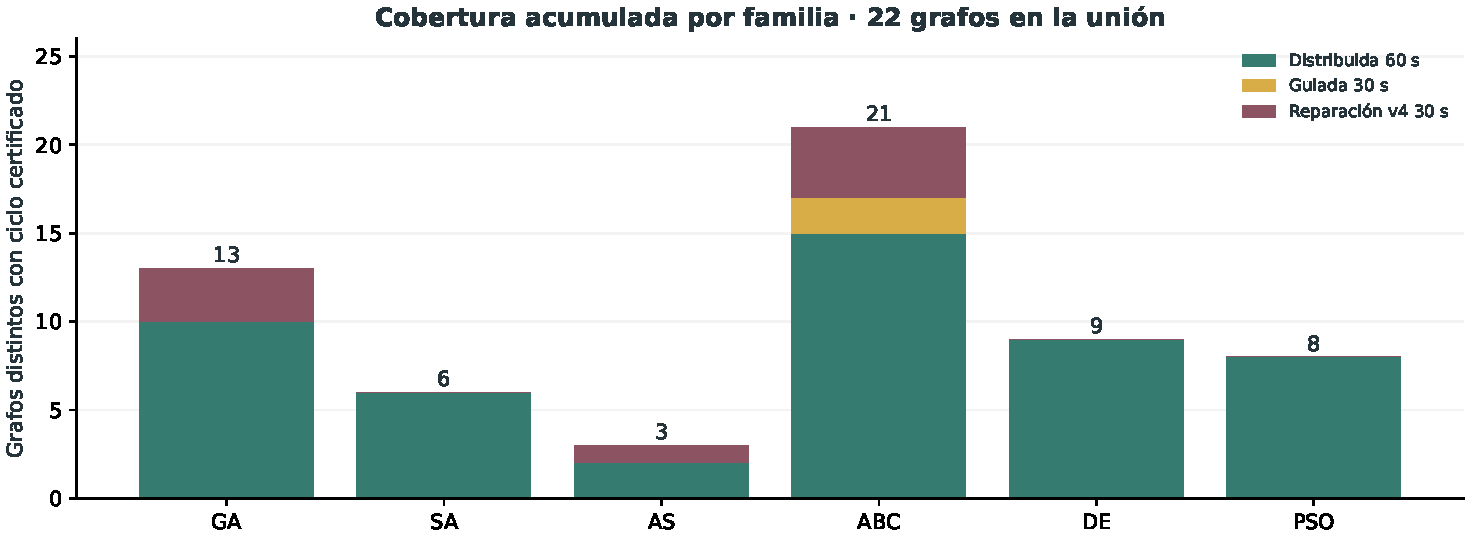
\includegraphics[width=\linewidth]{figures/exploratory-cumulative-coverage.pdf}
\caption{Grafos distintos certificados por familia a lo largo de las tres entregas. Cada color identifica el protocolo que añade el certificado. Las familias pueden resolver el mismo grafo: las barras se solapan en cobertura y no se suman para obtener los 22 grafos de la unión. No es una comparación de tasas ni tiempos entre protocolos.}\label{fig:cumulativecoverage}
\end{figure}

\subsection{Campaña inicial: límites observados}
La campaña inicial registró cero ciclos certificados en los 900 primarios de evaluación y escala, distribuidos en 150 intentos por familia. Hubo 630 agotamientos por plazo y 270 por evaluaciones, sin errores de ejecución ni timeouts externos en esos primarios. En 30 intentos de AS sobre graph1001 no se completó candidato y no se asignó costo ficticio.

\begin{table}[H]\centering\small
\caption{Resultados principales de la campaña histórica M6. Los límites efectivos son motivos de parada, no una prueba de imposibilidad.}\label{tab:historical}
\begin{tabularx}{\linewidth}{Yrrrr}
\toprule
Familia & Éxitos/150 & Plazos & Eval. límite & Sin candidato \\ \midrule
GA & 0/150 & 90 & 60 & 0 \\
SA & 0/150 & 90 & 60 & 0 \\
AS & 0/150 & 150 & 0 & 30 \\
ABC & 0/150 & 60 & 90 & 0 \\
DE & 0/150 & 120 & 30 & 0 \\
PSO & 0/150 & 120 & 30 & 0 \\
\bottomrule\end{tabularx}

\end{table}

AS mostró un cuello de botella de construcción: en la instancia de escala no terminó rutas completas. En graph48, las otras cinco familias alcanzaron las 10\,000 evaluaciones en todos los intentos; en graph479 y graph1001 todas las familias llegaron al plazo temporal. Un presupuesto máximo común no produjo el mismo número de evaluaciones efectivas. Las incidencias de swap y alimentación se preservaron en la campaña y limitaron las conclusiones temporales.

No existe un ganador por éxito en esta etapa. La coincidencia de los seis pares de verificación sustenta la reproducibilidad de rutas, costos, estados y contadores bajo su protocolo; no exige ni implica tiempos idénticos.

\subsection{Cobertura y resultados de la evaluación final}
La evaluación consolidada registra \TotalAttempts{} intentos: \TotalSuccesses{} éxitos certificados, \TotalExhausted{} agotamientos y \TotalErrors{} incidencias. La tasa descriptiva conjunta es \SuccessRate\%, incluidos los errores. Los éxitos corresponden a \SolvedGraphs{} grafos distintos, no a \TotalSuccesses{} grafos.

\begin{table}[H]\centering\small
\caption{Entrega por integrante. ``Completos'' indica 60 combinaciones conciliadas, no grafos resueltos. HC indica grafos distintos certificados.}\label{tab:members}
\begin{tabularx}{\linewidth}{Yrrrrr}
\toprule
Equipo & Intentos & Completos & Parciales & HC & Éxitos \\ \midrule
Arturo & 2\,417 & 40 & 1 & 4 & 72 \\
Elías & 600 & 10 & 0 & 1 & 13 \\
Eder & 2\,611 & 42 & 2 & 4 & 98 \\
Zapata & 1\,325 & 22 & 1 & 3 & 72 \\
César & 1\,853 & 30 & 1 & 3 & 90 \\
\bottomrule\end{tabularx}

\end{table}

De los 1001 candidatos, 852 no se iniciaron en las entregas. Entre los 149 iniciados se resolvieron 15 (10.07\%); este porcentaje describe el corte, no la probabilidad de resolver un grafo aleatorio del challenge. Los cinco parciales se mantienen identificados en el cuadro~\ref{tab:partial}.

\begin{table}[H]\centering\small
\caption{Grafos con cobertura parcial al cierre.}\label{tab:partial}
\begin{tabularx}{\linewidth}{lYrrr}
\toprule
Grafo & Equipo & Intentos & Pendientes & Incidencias \\ \midrule
104 & Zapata & 5 & 55 & 1 \\
153 & César & 53 & 7 & 1 \\
185 & Arturo & 17 & 43 & 1 \\
222 & Eder & 48 & 12 & 0 \\
227 & Eder & 43 & 17 & 0 \\
\bottomrule\end{tabularx}

\end{table}

\subsection{Comparación entre las seis familias}
El cuadro~\ref{tab:algorithms} restringe la comparación a los 144 grafos con cobertura completa. Todos los éxitos del corte se encuentran en ese grupo. El denominador es 1\,440 intentos por algoritmo; las nueve incidencias de ese grupo se conservan. Las tres incidencias restantes pertenecen a grafos parciales.

\begin{table}[H]\centering\small
\caption{Resultados en 144 grafos completos. Media: tiempo de proceso disponible, incluidos agotamientos e incidencias; combina ejecución serial y paralela.}\label{tab:algorithms}
\begin{tabularx}{\linewidth}{lYrrrr}
\toprule
Familia & Éxitos/intentos & Tasa (\%) & Grafos HC & Media (s) & Incid. \\ \midrule
GA & 70/1440 & 4.86 & 10 & 57.348 & 1 \\
SA & 18/1440 & 1.25 & 6 & 59.516 & 0 \\
AS & 14/1440 & 0.97 & 2 & 59.744 & 1 \\
ABC & 116/1440 & 8.06 & 15 & 55.897 & 2 \\
DE & 65/1440 & 4.51 & 9 & 57.428 & 4 \\
PSO & 62/1440 & 4.31 & 8 & 57.655 & 1 \\
\bottomrule\end{tabularx}

\end{table}

ABC alcanzó los 15 grafos certificados y produjo 116 éxitos por intento. GA alcanzó diez grafos, DE nueve, PSO ocho, SA seis y AS dos. Estos conteos se solapan: su suma no es el número de grafos distintos del equipo. En este corte ABC tuvo la mayor cobertura y frecuencia de éxito, aunque su tasa por intento fue menor de 9\% bajo la cobertura balanceada.

\begin{figure}[H]\centering
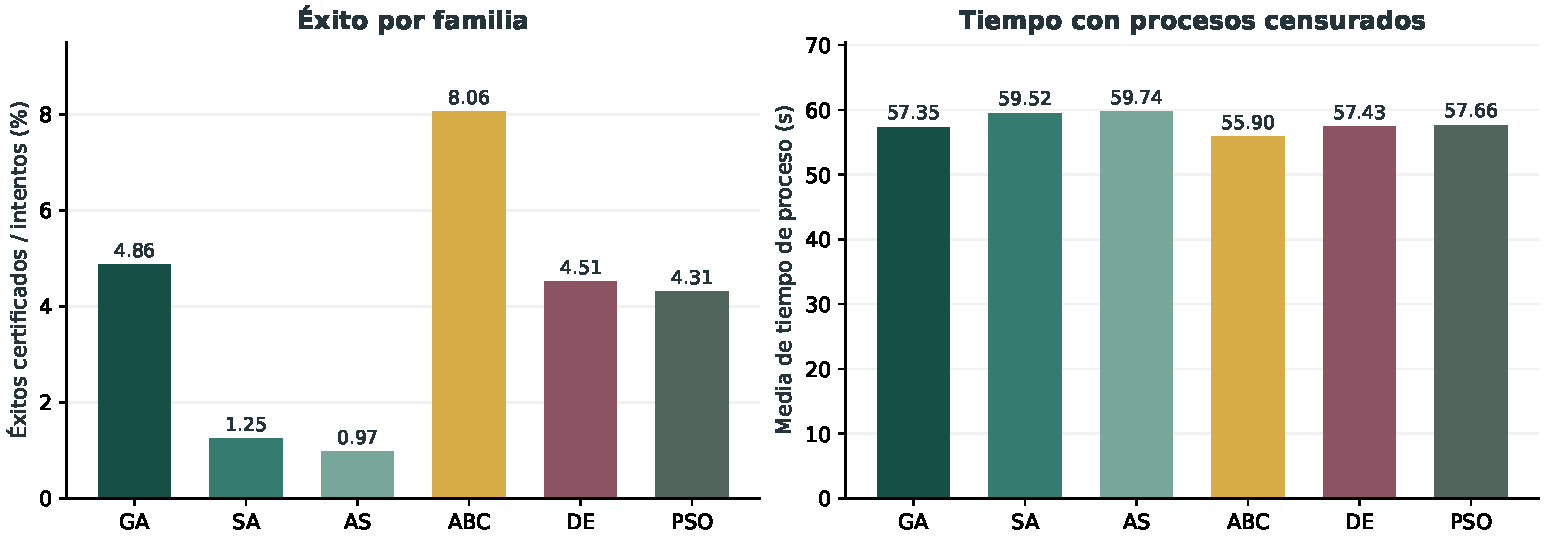
\includegraphics[width=\linewidth]{figures/performance.pdf}
\caption{Éxito y tiempo descriptivos con cobertura completa. Las medias incorporan procesos sin solución que agotaron el plazo; no equivalen a tiempos medios hasta éxito.}\label{fig:performance}
\end{figure}

Las medias están próximas al plazo por los agotamientos. Más éxitos tempranos pueden reducir la media sin implicar mayor rapidez cuando no se resuelve. Se incluyen arranque/carga y se mantienen los tiempos faltantes; la mezcla de ejecución serial y paralela impide interpretarlo como un orden de eficiencia.

\subsection{Distribución de tiempos y costos}
Las figuras~\ref{fig:timeboxes} y~\ref{fig:costboxes} complementan las medias con diagramas de cajas por familia. Se utilizan los 144 grafos completos, separando ejecución serial y paralela. Cada etiqueta indica el número de observaciones disponibles; no se imputan tiempos ni costos ausentes. Los paneles tienen subconjuntos de instancias y equipos diferentes, por lo que no son una comparación controlada entre modos.

\begin{figure}[H]\centering
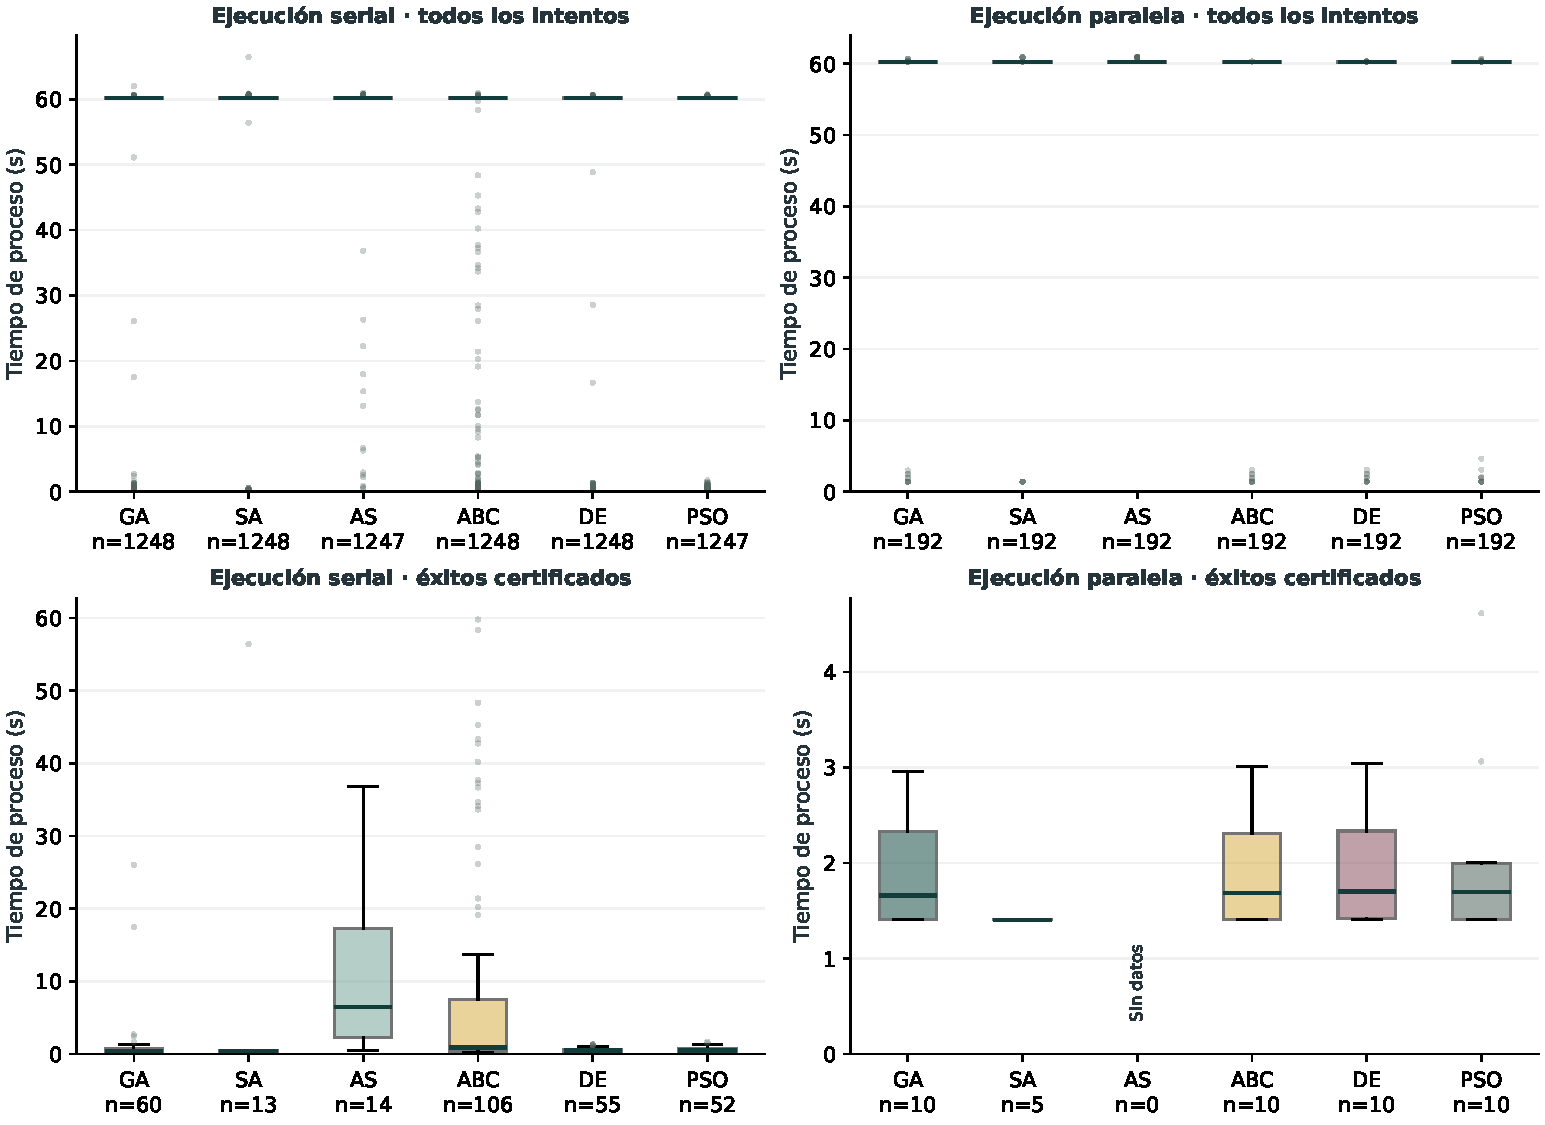
\includegraphics[width=\linewidth]{figures/runtime-boxplots.pdf}
\caption{Distribución de tiempos de proceso. Arriba: todos los intentos con duración disponible, incluidos agotamientos e incidencias. Abajo: únicamente éxitos certificados, un subconjunto condicionado a resolver. La caja abarca los percentiles 25--75, la línea indica la mediana y los bigotes llegan hasta los valores observados dentro de 1.5 rangos intercuartílicos; los puntos exteriores no se eliminan.}\label{fig:timeboxes}
\end{figure}

La concentración de cajas cerca de 60 segundos refleja el presupuesto y la censura de las búsquedas sin éxito. Los puntos rápidos pueden corresponder a soluciones tempranas o incidencias; el panel de éxitos los distingue sin convertir su distribución en tiempo general hasta solución. Una caja estrecha no demuestra robustez fuera de este corte. Los paneles vacíos indican ausencia de éxitos y no tiempo cero.

\begin{figure}[H]\centering
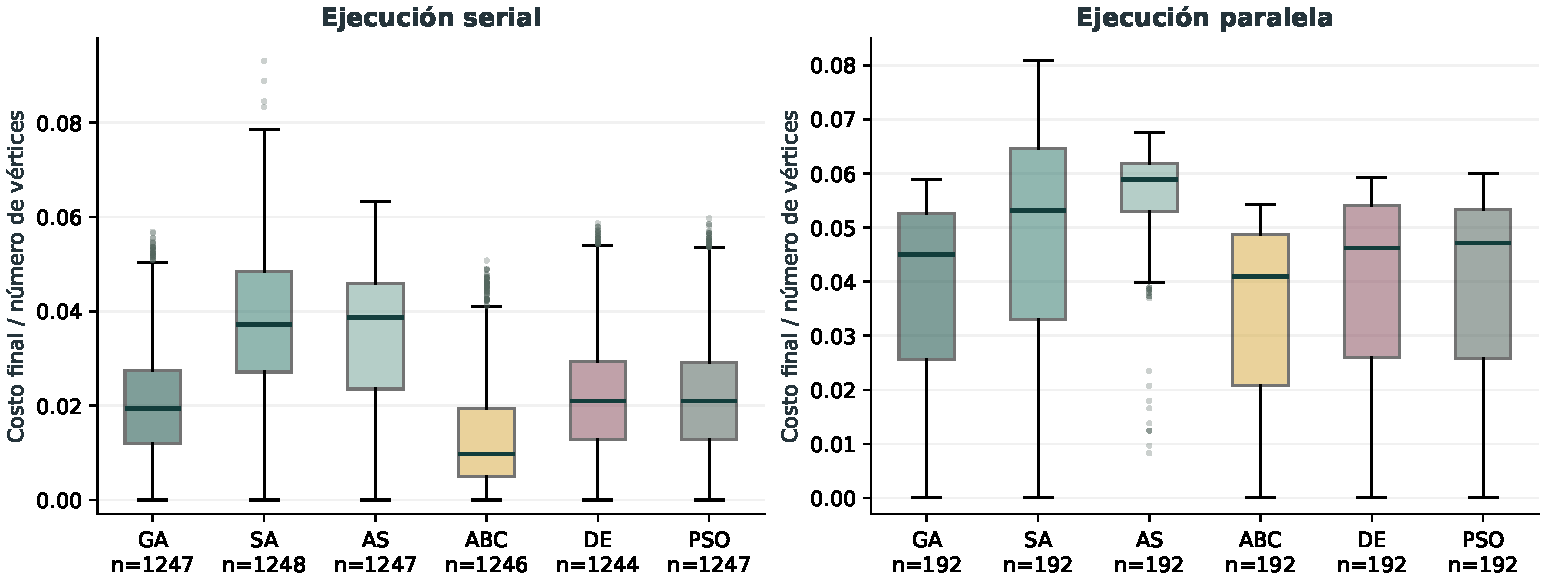
\includegraphics[width=\linewidth]{figures/cost-boxplots.pdf}
\caption{Distribución del mejor costo final por intento, dividido entre el número de vértices, con la misma convención de cajas y bigotes. Se incluyen los candidatos disponibles de los grafos completos, con y sin éxito. Un valor cero requiere además el certificado independiente.}\label{fig:costboxes}
\end{figure}

La normalización facilita mostrar grafos de tamaños distintos, pero no iguala su dificultad estructural. Un costo positivo pequeño sigue siendo una ruta sin ciclo certificado. Los cuartiles, bigotes, tamaños de muestra y cantidad de puntos exteriores se exportan en \code{docs/latex/tables/boxplot-statistics.csv}.

\subsection{Los 22 grafos certificados y variación entre semillas}
El cuadro~\ref{tab:solved} incluye los 22 grafos distintos certificados en las entregas. Para cada grafo muestra el protocolo en el que se obtuvo su primer certificado y los éxitos/intentos de esa misma evaluación. La figura~\ref{fig:heatmap} conserva ese criterio por familia y explicita los denominadores: cinco intentos en los dos grafos de la exploración guiada y diez en las otras filas. La selección y los presupuestos difieren, por lo que las celdas describen los registros y no una comparación controlada entre protocolos.

\begin{table}[H]\centering\small
\caption{Los 22 grafos distintos certificados en el conjunto de entregas. El denominador corresponde a los intentos admitidos en el protocolo indicado, incluidas incidencias; los éxitos pueden proceder de varias familias.}\label{tab:solved}
\begin{tabularx}{\linewidth}{lrYr}
\toprule
Grafo & Vértices & Protocolo del certificado & Éxitos/intentos \\ \midrule
1 & 66 & Reparación v4 30 s & 3/60 \\
2 & 70 & Distribuida 60 s & 26/60 \\
4 & 84 & Guiada 30 s & 1/30 \\
6 & 94 & Distribuida 60 s & 20/60 \\
10 & 118 & Distribuida 60 s & 13/60 \\
14 & 142 & Distribuida 60 s & 9/60 \\
18 & 166 & Distribuida 60 s & 6/60 \\
23 & 190 & Distribuida 60 s & 5/60 \\
27 & 214 & Distribuida 60 s & 6/60 \\
31 & 238 & Distribuida 60 s & 2/60 \\
35 & 262 & Guiada 30 s & 1/30 \\
39 & 286 & Reparación v4 30 s & 1/60 \\
43 & 310 & Reparación v4 30 s & 2/60 \\
47 & 334 & Reparación v4 30 s & 2/60 \\
52 & 358 & Reparación v4 30 s & 3/60 \\
56 & 382 & Distribuida 60 s & 1/60 \\
72 & 460 & Distribuida 60 s & 44/60 \\
79 & 480 & Distribuida 60 s & 43/60 \\
90 & 510 & Distribuida 60 s & 41/60 \\
96 & 540 & Distribuida 60 s & 44/60 \\
134 & 724 & Distribuida 60 s & 45/60 \\
150 & 823 & Distribuida 60 s & 40/60 \\
\bottomrule\end{tabularx}

\end{table}

\begin{figure}[H]\centering
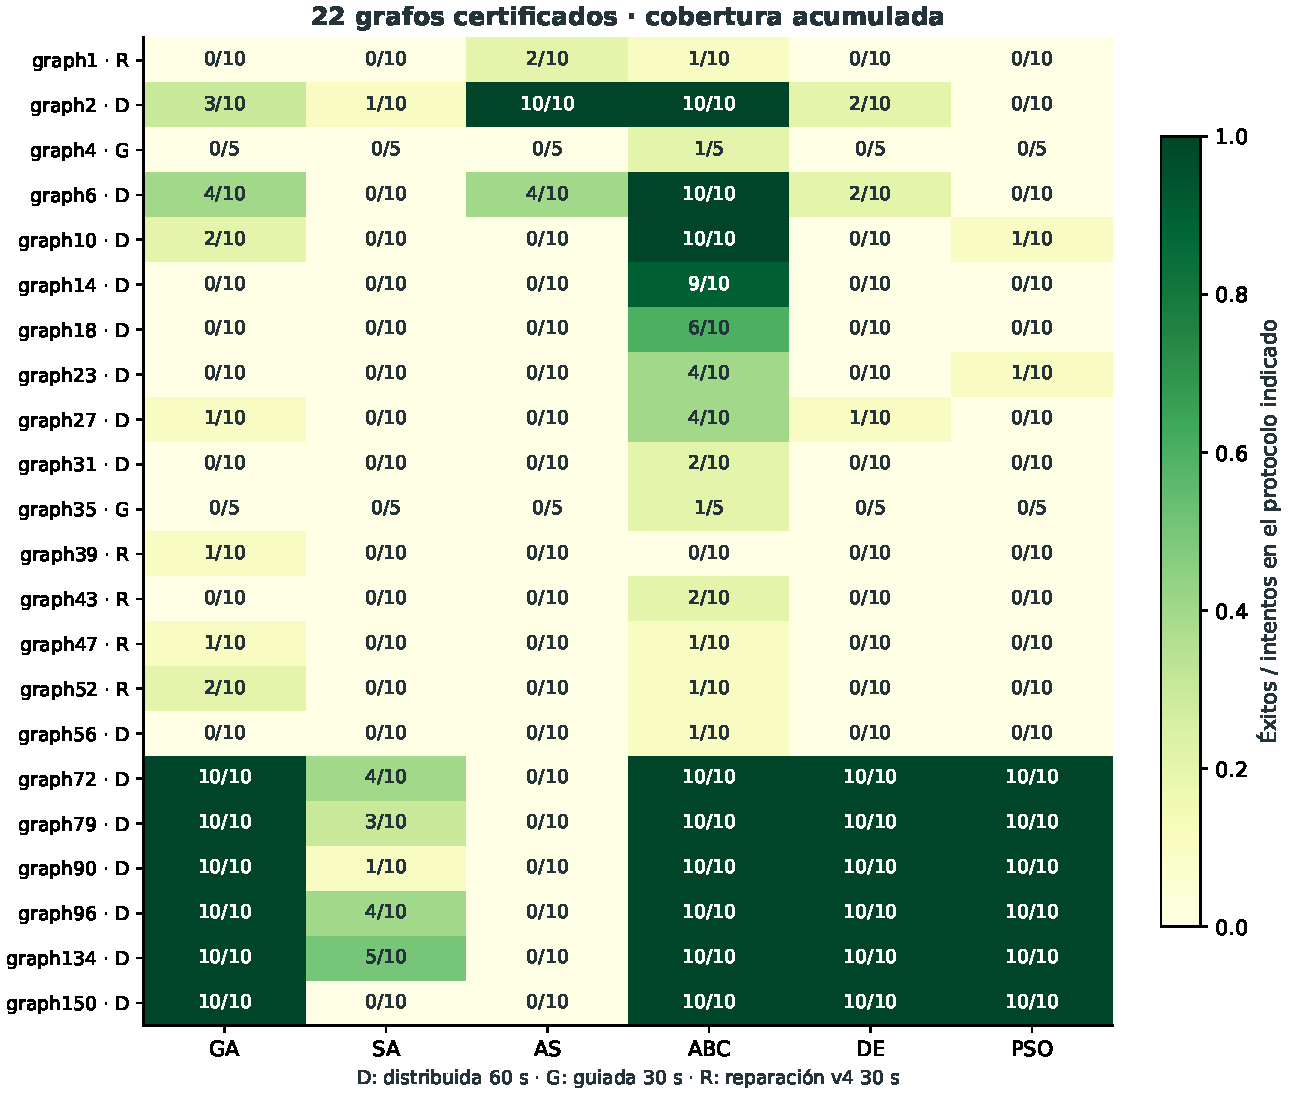
\includegraphics[width=.98\linewidth]{figures/exploratory-cumulative-heatmap.pdf}
\caption{Los 22 grafos certificados. Cada celda muestra éxitos/intentos de la familia en el protocolo indicado en la fila: D, distribuida (60 s); G, exploración guiada (30 s); R, reparación v4 (30 s). El color representa esa fracción dentro de su propio protocolo. No se mezclan intentos de configuraciones distintas ni se extrapola al challenge completo.}\label{fig:heatmap}
\end{figure}

\subsection{Calidad de candidatos y escala}
La figura~\ref{fig:cost} muestra el menor costo normalizado observado por grafo iniciado en cualquiera de las tres entregas, incluidos los resultados recientes. Los 22 grafos certificados aparecen en cero; los valores positivos indican transiciones ausentes. Un costo pequeño puede significar cercanía en esta función objetivo y, aun así, no cumplir el cierre. El eje de vértices se presenta en escala logarítmica para conservar legibilidad entre tamaños.

\begin{figure}[H]\centering
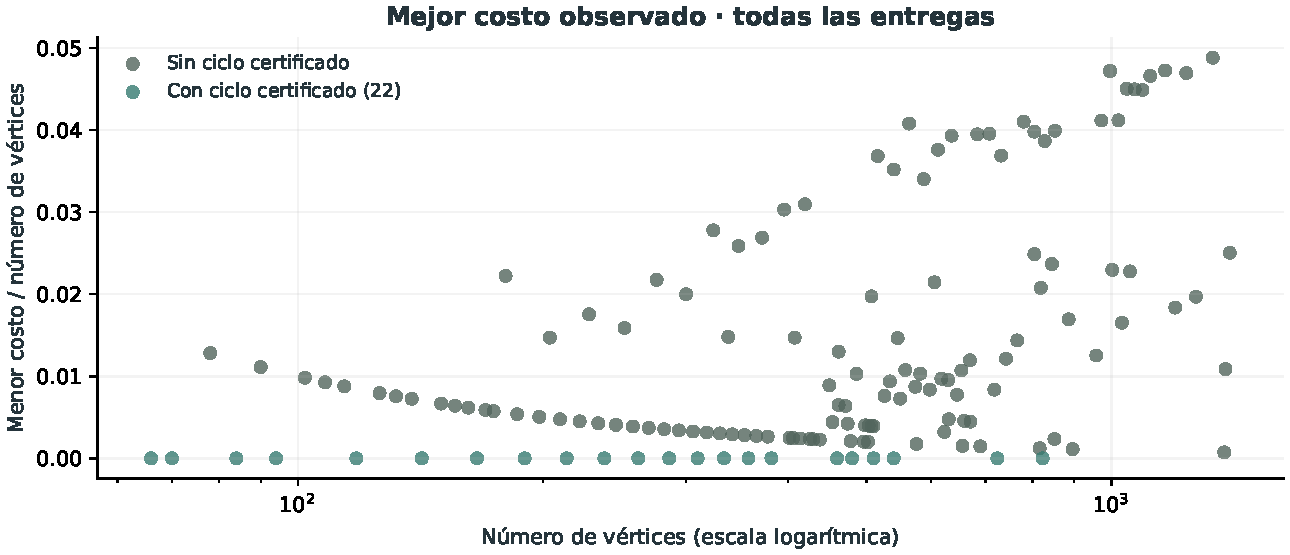
\includegraphics[width=\linewidth]{figures/exploratory-cumulative-cost.pdf}
\caption{Mejor costo acumulado entre las entregas para los 149 grafos iniciados, con 22 ciclos certificados. Se toma el mínimo disponible por ID sin sumar costos ni equiparar presupuestos; las instancias tienen distinta cobertura de intentos y configuraciones.}\label{fig:cost}
\end{figure}

La figura no identifica causalidad: tamaño, estructura, hardware, políticas y cobertura cambian conjuntamente. No se extrapola a los 852 grafos sin iniciar.

\subsection{Incidencias preservadas}
Se preservaron tres interrupciones de Arturo, seis de Zapata, dos de César y una de Eder, sin reintentos automáticos. Los 600 primarios de Elías pudieron recuperarse y auditarse pese al fallo de longitud de ruta y los huecos de su historial de sesiones.

\pagina{Cierre de las evaluaciones exploratorias}
\label{sec:exploration}
\subsection{Selección dirigida y cierre de la entrega}
Se cerraron dos exploraciones complementarias a la evaluación distribuida. La primera utilizó las variantes guiadas en doce grafos reportados como resueltos por otro equipo y sin certificado en nuestro consolidado. Registró \PriorAttempts{} intentos, dos éxitos certificados y \PriorErrors{} interrupciones; encontró ciclos en graph4 y graph35. Se conserva como un protocolo separado de la evaluación distribuida.

La exploración v4 seleccionó 65 grafos todavía pendientes: 41 con mejor costo previo uno, 15 con costo dos y siete con costo tres, además de graph99 y graph85, con costos cuatro y cinco, que el otro equipo reportó resueltos. Se eliminaron duplicados y se excluyeron graph4 y graph35 por sus certificados ya disponibles. El costo previo procede de la evaluación distribuida, no de una distancia garantizada a una solución.

El protocolo fijó seis familias, diez semillas 2001--2010, hasta 30 segundos por intento y cuatro procesos independientes, con un hilo nativo por proceso y afinidad a las CPU lógicas 0, 2, 4 y 6 de la laptop de Arturo. No hubo límite de evaluaciones ni iteraciones; el límite externo fue de 90 segundos para incluir arranque y carga. Se admitió solo un intento simultáneo del mismo grafo. El orden priorizó los diez éxitos externos pendientes y después el costo previo.

La evaluación quedó cerrada en \RepairAttempts{} de las 3\,900 combinaciones previstas (\RepairCoverage\%). Se conservaron \RepairSuccesses{} éxitos, \RepairExhausted{} agotamientos y \RepairErrors{} interrupciones. Alcanzó \RepairStarted{} grafos: \RepairComplete{} completos y \RepairPartial{} parciales; otros \RepairUnstarted{} no se iniciaron. Las \RepairOmitted{} combinaciones no ejecutadas quedan fuera de la entrega y no se retomarán. Las incidencias del cierre permanecen en el denominador.

La sesión registrada duró \RepairSessionHours{} horas de reloj. Esta duración incluye coordinación y cuatro procesos concurrentes; no es una duración serial ni acredita aceleración frente a las etapas anteriores. Se volvieron a auditar los \RepairAttempts{} registros v4 y los \PriorAttempts{} de la exploración previa, comprobando artefactos, identidades, costo y ciclos sin ejecutar nuevamente los algoritmos.

\subsection{Éxitos y cobertura de los algoritmos}
La reparación v4 certificó cinco grafos adicionales: graph1, graph39, graph43, graph47 y graph52. El cuadro~\ref{tab:repairfamilies} conserva todos los intentos, mientras que su tasa balanceada y mediana temporal utilizan únicamente los \RepairComplete{} grafos completos: \RepairBalancedDenominator{} intentos por familia. Los cuatro parciales no alteran ese denominador.

\begin{table}[H]\centering\small
\caption{Cierre v4 por familia. Intentos, éxitos e incidencias corresponden al total; HC cuenta grafos distintos. Tasa balanceada y mediana de proceso usan los 48 grafos completos.}\label{tab:repairfamilies}
\begin{tabularx}{\linewidth}{Yrrrrrr}
\toprule
Familia & Intentos & Éxitos & Incid. & HC & Tasa bal. (\%) & Mediana (s) \\ \midrule
GA & 498 & 4 & 1 & 3 & 0.83 & 30.86 \\
SA & 497 & 0 & 1 & 0 & 0.00 & 30.86 \\
AS & 496 & 2 & 0 & 1 & 0.42 & 30.86 \\
ABC & 496 & 5 & 1 & 4 & 1.04 & 30.86 \\
DE & 495 & 0 & 1 & 0 & 0.00 & 30.86 \\
PSO & 494 & 0 & 0 & 0 & 0.00 & 30.86 \\
\bottomrule\end{tabularx}

\end{table}

ABC produjo cinco éxitos en cuatro grafos, GA cuatro éxitos en tres grafos y AS dos éxitos en un grafo. Sus coberturas se solapan: no se suman para obtener cinco grafos distintos. SA, DE y PSO no certificaron ciclos en esta exploración. Esos resultados no invalidan sus éxitos bajo el protocolo distribuido de 60 segundos y otra configuración.

\begin{figure}[H]\centering
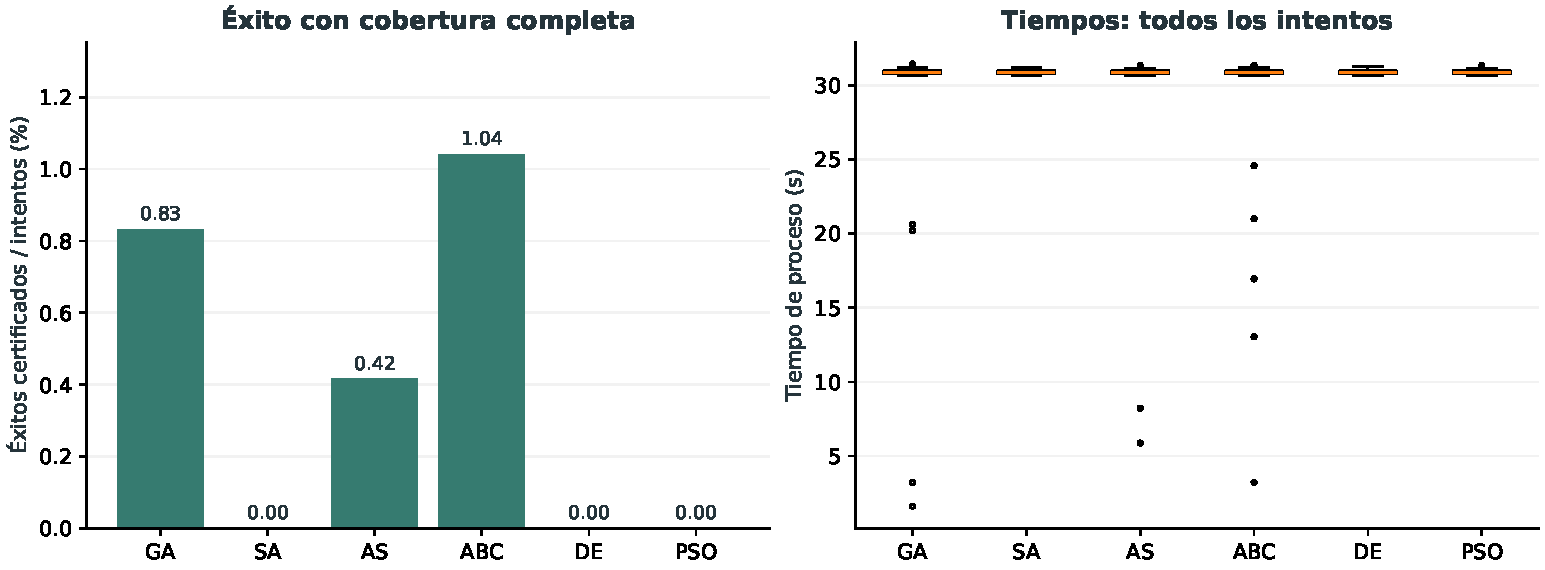
\includegraphics[width=\linewidth]{figures/exploratory-performance.pdf}
\caption{Exploración v4 en grafos completos: tasa de éxito y cajas de tiempo de proceso, con 480 observaciones por familia. Los tiempos incluyen intentos agotados; la mediana cercana al plazo no es un tiempo medio hasta resolver. Cajas: percentiles 25--75; bigotes: valores dentro de 1.5 rangos intercuartílicos; puntos exteriores conservados.}\label{fig:repairperformance}
\end{figure}

\begin{figure}[H]\centering
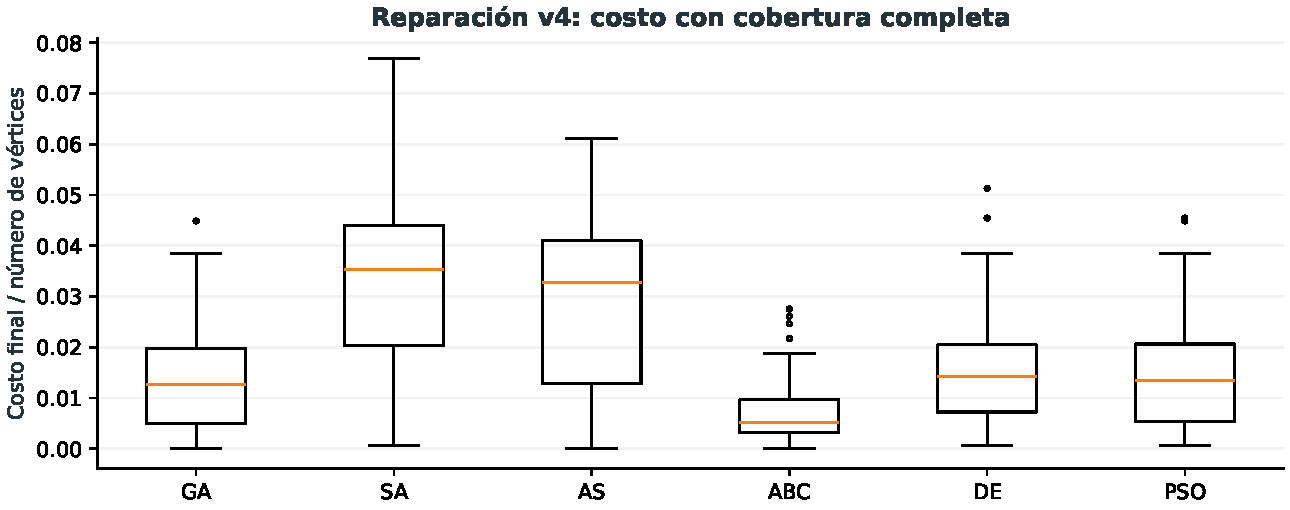
\includegraphics[width=.94\linewidth]{figures/exploratory-cost-boxplots.pdf}
\caption{Costo final normalizado por vértices en los mismos 48 grafos completos, con 480 candidatos por familia. Un costo positivo, aunque pequeño, no constituye ciclo. La convención de cajas es la de la figura~\ref{fig:repairperformance}.}\label{fig:repaircost}
\end{figure}

Los 41 grafos seleccionados por costo previo uno completaron sus 60 combinaciones. También se completaron los diez grafos pendientes reportados como resueltos por el otro equipo: cinco recibieron certificado propio; graph8, graph67, graph78, graph85 y graph99 agotaron sus combinaciones sin éxito. Los CSV externos aportan éxito declarado y dimensiones, pero no rutas para certificar sus soluciones ni condiciones equivalentes para comparar tasas.

Los parciales del cierre fueron graph60 (26 intentos), graph61 (25), graph66 (23) y graph71 (22). Quedaron sin iniciar graph77, graph83, graph86, graph88, graph89, graph115, graph154, graph25, graph73, graph76, graph117, graph123 y graph126. El anexo conserva costo previo/final y cobertura para los 65 seleccionados; no se presentan los no ejecutados como fallos.

\subsection{Balance de la entrega y límites de interpretación}
\begin{table}[H]\centering\small
\caption{Resultados por protocolo. Las filas conservan sus propios presupuestos y denominadores; no se calcula una tasa de éxito conjunta.}\label{tab:stagesclosed}
\begin{tabularx}{\linewidth}{Yrrr}
\toprule
Etapa & Intentos & Éxitos & Grafos HC \\ \midrule
M6: evaluación y escala & 900 & 0 & 0 \\
Evaluación distribuida & 8\,806 & 345 & 15 \\
Exploración guiada & 118 & 2 & 2 \\
Exploración con reparación v4 & 2\,976 & 11 & 5 \\
\bottomrule\end{tabularx}

\end{table}

\begin{table}[H]\centering\small
\caption{Siete grafos adicionales certificados en las exploraciones, ausentes del conjunto de 15 resueltos de la evaluación distribuida. Los conteos son intentos exitosos.}\label{tab:exploratorysolved}
\begin{tabularx}{\linewidth}{lYY}
\toprule
Grafo & Exploración & Éxitos por familia \\ \midrule
4 & Guiada & ABC: 1 \\
35 & Guiada & ABC: 1 \\
1 & Reparación v4 & ABC: 1, AS: 2 \\
39 & Reparación v4 & GA: 1 \\
43 & Reparación v4 & ABC: 2 \\
47 & Reparación v4 & ABC: 1, GA: 1 \\
52 & Reparación v4 & ABC: 1, GA: 2 \\
\bottomrule\end{tabularx}

\end{table}

La unión de los 15 grafos de la evaluación distribuida, los dos de la exploración guiada y los cinco de v4 contiene \UnionCertifiedGraphs{} grafos distintos certificados. Se superó así la referencia aproximada de 20 al considerar el conjunto de entregas, aunque la evaluación distribuida por sí sola conservó 15. La meta original de 60 no se alcanzó. La unión expresa cobertura acumulada, no una tasa comparable entre protocolos.

La selección se basó en resultados previos y éxitos externos; por tanto, presenta sesgo de selección y reutilización. Cambiaron operadores, semillas, presupuesto y concurrencia respecto a la evaluación distribuida. Los cinco ciclos adicionales demuestran soluciones válidas bajo v4, pero no aíslan el efecto causal de la reparación ni prueban superioridad estadística general. La ausencia de ciclos en otros intentos tampoco demuestra no hamiltonicidad.

\pagina{Contraste con resultados publicados del FHCP}
El contraste bibliográfico reutiliza el inventario y los localizadores verificados de M6. Las fuentes primarias no proporcionan condiciones equivalentes a nuestras ejecuciones: difieren métodos, instancias, presupuestos, equipos y repeticiones. Siguiendo buenas prácticas de comparación de optimización, esas diferencias se explicitan antes de interpretar cifras \citep{beiranvand2017BestPractices}.

\subsection{Cobertura del concurso y dificultad estructural}
El portal oficial informa que Cohen y Coudert presentaron ciclos para 985 de los 1001 grafos del concurso \citep{flindersFhcpChallenge}. Ese resultado es cobertura acumulada durante una ventana de concurso; no equivale a diez o treinta semillas con un plazo individual homogéneo. Comparar su porcentaje directamente con 15 de 149 grafos iniciados produciría una equivalencia que los datos no sostienen.

La construcción del conjunto consideró dificultad para Concorde, LKH y SLH, seleccionando candidatos problemáticos para al menos dos de esos métodos \citep{haythorpe2018Fhcp}. Esta procedencia ayuda a interpretar por qué un constructor o movimiento local puede estancarse, pero no aporta por sí sola una matriz temporal reproducible para esos tres solvers. Los tours oficiales sirven como referencias de soluciones conocidas y no como mediciones propias de rendimiento.

\subsection{Contraste por instancia y tipo de salida}
Cohen y Coudert describen un oráculo de programación entera con SageMath y CPLEX y publican tiempos puntuales para algunos IDs; graph1 y graph2 aparecen con 0.76 y 0.01 segundos \citep{cohenCoudert2017Challenge}. No se precisan todas las condiciones necesarias para una comparación temporal equivalente. En nuestra campaña histórica, los IDs compartidos pertenecían a comprobación o verificación, no a evaluación final; el CSV trazable conserva esa distinción en 36 contrastes.

HybridHAM combina construcción voraz, transformaciones por rotación y criterios de alcanzabilidad \citep{seeja2018HybridHam}. Su tabla diferencia HP y HC: graph1 aparece como camino con 0.0625 segundos y graph2 como ciclo con 0.0469. El artículo indica Core i5, 4 GB de RAM y MATLAB 13RA, sin especificar todas las condiciones de repetición y presupuesto requeridas para comparar con nuestro entorno.

Además, su texto de la sección 4.3 declara seis ciclos entre 250 instancias y 75 caminos, mientras la tabla 4 etiqueta más de seis instancias como HC. Se conserva esa discrepancia interna y no se infiere un total corregido ni una tasa global. Los tiempos por ID se atribuyen a las filas correspondientes; no se convierte un HP en ciclo para aumentar el éxito publicado.


\pagina{Discusión, cuellos de botella y limitaciones}
\subsection{Interpretación de los cambios}
La campaña inicial evidenció que preservar permutaciones no basta para encontrar ciclos. Introducir información de adyacencia reduce parte del trabajo ciego, pero decisiones localmente favorables pueden ser incompatibles con el cierre global.

La etapa posterior cambió políticas, tiempo por intento y reparto de hardware. La diferencia entre cero éxitos históricos y 15 grafos finales no estima el efecto causal de un componente. Para atribuir efectos a inicialización, guía, recalentamiento o costo incremental se necesita una ablación con iguales instancias, semillas, equipos y presupuestos.

\subsection{Familia mejor adaptada al corte}
ABC presentó la mayor cobertura observada: alcanzó los 15 grafos resueltos y 116 éxitos en 1\,440 intentos sobre cobertura completa. La explotación de fuentes, renovación por abandono y vecindades guiadas son compatibles con ese comportamiento, pero el experimento no aísla el aporte de cada mecanismo. La conclusión es descriptiva y corresponde a la configuración evaluada.

GA, DE y PSO también produjeron ciclos; la menor cobertura de SA no descarta otros esquemas de temperatura o vecindad. En AS persiste el costo de construir rutas y actualizar feromonas, sin perfilado suficiente para cuantificar cada operación. No se supone equivalencia de trabajo entre una evaluación incremental, la construcción de una ruta y la decodificación de claves de una población.

\subsection{Validez y trabajo futuro}
La selección final contiene prefijos de colas asignadas, con instancias reutilizadas durante el desarrollo y máquinas diferentes. No es representativa de los 1001 grafos. Los éxitos entre semillas del mismo grafo no se tratan como observaciones independientes para sostener una superioridad estadística general.

Los parciales quedan fuera de la tabla balanceada pero dentro de los totales. La censura por plazo, los tiempos faltantes y los historiales incompletos impiden estimar un tiempo calendario o medio hasta solución fiable. Certificados, hashes y reproducción reducen errores de medición; no eliminan sesgos de selección ni garantizan resultados futuros.

Las exploraciones cerradas añaden siete grafos certificados a los 15 de la evaluación distribuida: dos con la variante guiada y cinco con reparación v4. La cobertura acumulada de \UnionCertifiedGraphs{} grafos supera la referencia aproximada de 20, pero no la meta original de 60. Cada etapa conserva su propio denominador y las combinaciones no ejecutadas quedan fuera de la entrega, sin continuación prevista.

En v4 solo ABC, GA y AS aportaron éxitos. La selección dirigida y los cambios simultáneos impiden generalizar ese orden al challenge o aislar efectos causales; no se realizaron ablaciones.

\pagina{Conclusiones}
Se implementaron las seis familias requeridas con un contrato común de ejecución y una representación que preserva permutaciones. La función de costo cuenta aristas faltantes, incluido el cierre; el éxito requiere un ciclo certificado y no solo una ruta bien formada o un fitness favorable.

La campaña histórica completó su protocolo y expuso límites de las variantes iniciales: cero éxitos en 900 primarios de evaluación y escala. Las mejoras posteriores y su evaluación independiente produjeron \TotalSuccesses{} éxitos en \TotalAttempts{} intentos y \SolvedGraphs{} grafos distintos certificados. Son etapas de condiciones diferentes que se conservan separadas, sin adjudicar la mejora a un único cambio.

ABC fue la familia que mejor se adaptó al corte observado por cobertura y éxitos: alcanzó los 15 grafos resueltos, con 116 éxitos en 1\,440 intentos sobre cobertura completa. Esta conclusión se restringe a las instancias, parámetros y recursos evaluados. Los tiempos cercanos al plazo, los equipos distintos y los agotamientos impiden sostener una superioridad temporal universal.

Las exploraciones complementarias certificaron graph4 y graph35 con la variante guiada y graph1, graph39, graph43, graph47 y graph52 con reparación v4. La evaluación v4 quedó cerrada en \RepairAttempts{} intentos, con \RepairSuccesses{} éxitos y \RepairErrors{} interrupciones, sobre \RepairComplete{} grafos completos y \RepairPartial{} parciales. ABC, GA y AS aportaron los ciclos de ese protocolo. La reparación produjo soluciones válidas en esta selección, sin que el diseño permita aislar su efecto causal.

El contraste FHCP se apoyó en fuentes primarias, distinguiendo caminos de ciclos y señalando presupuestos y condiciones ausentes. No se presentaron las referencias oficiales ni las publicaciones como ejecuciones propias, ni se calcularon aceleraciones entre entornos no equivalentes.

La unión de las entregas contiene \UnionCertifiedGraphs{} grafos distintos certificados, por encima de la referencia aproximada de 20 y por debajo de la meta original de 60. La evaluación distribuida conserva sus cinco parciales, 12 incidencias y 51\,254 combinaciones fuera de alcance; v4 conserva otras \RepairOmitted{} combinaciones no ejecutadas. Estos conteos pertenecen a planes diferentes y no se suman como cobertura homogénea. Se cierra la entrega en los cortes documentados, sin retomar las corridas omitidas. El principal aporte es una comparación verificable de implementaciones reales, con datos recuperables y tablas/figuras regenerables, además de conclusiones ajustadas al alcance de la evidencia.

\clearpage\phantomsection\addcontentsline{toc}{section}{Referencias}
\renewcommand{\refname}{Referencias}
\begingroup\footnotesize\singlespacing\raggedright
\bibliographystyle{plainnat}\bibliography{bibliography/references}
\endgroup
\appendix
\pagina{Parámetros y trazabilidad}
\label{sec:parameters}
Los valores siguientes proceden del plan compartido de la evaluación final. No son parámetros inferidos de las tablas ni una configuración retrospectivamente elegida por sus éxitos.
\begingroup\small\setlength{\tabcolsep}{4pt}\begin{tabularx}{\linewidth}{lY}
\toprule
Familia & Parámetros efectivos \\ \midrule
GA & \ttfamily\footnotesize crossover\_rate=0.8; elite\_count=1; guided\_move\_rate=0.5; initialization=greedy; mutation\_rate=0.1; population\_size=20; tournament\_size=3 \\
SA & \ttfamily\footnotesize cooling\_factor=0.95; cost\_mode=incremental; guided\_move\_rate=0.5; incremental\_check\_interval=1000; initial\_temperature=2.0; initialization=greedy; minimum\_temperature=1e-06; moves\_per\_temperature=50; reheat\_after=1000 \\
AS & \ttfamily\footnotesize alpha=1.0; ant\_count=20; beta=4.0; construction=neighbor\_guided; epsilon=0.05; initial\_pheromone=1.0; pheromone\_max=10.0; pheromone\_min=0.1; pheromone\_storage=edges; q=1.0; rho=0.2 \\
ABC & \ttfamily\footnotesize cost\_mode=incremental; guided\_move\_rate=0.5; incremental\_check\_interval=1000; initialization=greedy; limit=200; source\_count=20 \\
DE & \ttfamily\footnotesize crossover\_rate=0.8; differential\_weight=0.8; initialization=greedy; population\_size=20 \\
PSO & \ttfamily\footnotesize cognitive\_coefficient=1.0; inertia=0.5; initialization=greedy; social\_coefficient=1.0; swarm\_size=20; velocity\_limit=0.5 \\
\bottomrule\end{tabularx}
\endgroup
\subsection{Identificadores de ejecución}
Campaña inicial: \code{e390b61f-aae4-4248-ba71-4467920d7bac}; código \code{22994034acb6eb4232fb72489758b6092cb0c626}. Evaluación final: \code{45f464ae-50be-441b-b7ff-a261fba5028e}; código \code{19ac5eaa46fbacc5a034dae6d14befbf171928db}. Los identificadores completos y hashes permiten distinguir las condiciones de ambas etapas.

Exploración guiada: \code{8d8c7fdd-0754-4515-ab98-e14548c63ae6}. Reparación v4: \code{ee2c634a-f402-486a-959c-44792cca616c}. Sus fuentes se identifican con hashes y snapshots, incluidos los cambios locales v4. El corte cerrado conserva planes, entorno, sesiones, intentos y certificados en \code{experiments/analysis/closed-explorations-20261117/}.

El manifiesto de figuras y tablas del informe registra el SHA-256 de cada entrada y salida en \code{docs/latex/asset-manifest.json}. Las figuras se generan con \code{scripts/build_report_assets.py}; no se transcriben cifras de forma manual.
\subsection{Reproducción del informe}
Generar activos desde la raíz con \code{python scripts/build_report_assets.py}. Desde \code{docs/latex}, compilar con:
\begin{quote}\footnotesize\ttfamily\raggedright
latexmk -pdf -interaction=nonstopmode -halt-on-error -outdir=build report.tex
\end{quote}
Las figuras requieren las dependencias de análisis fijadas; la compilación requiere TeX Live con español, \code{latexmk}, pdfLaTeX y BibTeX. La guía \code{docs/latex/README.md} detalla comprobaciones y destinos. Esta reproducción no ejecuta solvers.
\pagina{Detalle por grafo evaluado}
Cada fila conserva las combinaciones admitidas, incluidos errores. Una fila con 60 intentos significa cobertura conciliada, no necesariamente 60 búsquedas terminadas normalmente ni un ciclo encontrado. Los 852 grafos sin iniciar permanecen en el CSV completo del repositorio y no se presentan como fracasos.
\begingroup\setstretch{1.0}\small\begin{longtable}{llrrrrr}
\caption{Cobertura de cada grafo iniciado. Los pendientes no son fallos.}\label{tab:allgraphs}\\
\toprule Grafo & Equipo & $n$ & Intentos & Éxitos & Incid. & Pend. \\ \midrule\endfirsthead
\toprule Grafo & Equipo & $n$ & Intentos & Éxitos & Incid. & Pend. \\ \midrule\endhead
\midrule\multicolumn{7}{r}{Continúa en la página siguiente}\endfoot\bottomrule\endlastfoot
1 & Arturo & 66 & 60 & 0 & 0 & 0 \\
2 & Zapata & 70 & 60 & 26 & 0 & 0 \\
3 & César & 78 & 60 & 0 & 0 & 0 \\
4 & Eder & 84 & 60 & 0 & 0 & 0 \\
5 & Elías & 90 & 60 & 0 & 0 & 0 \\
6 & Arturo & 94 & 60 & 20 & 0 & 0 \\
7 & Zapata & 102 & 60 & 0 & 3 & 0 \\
8 & César & 108 & 60 & 0 & 0 & 0 \\
9 & Eder & 114 & 60 & 0 & 0 & 0 \\
10 & Elías & 118 & 60 & 13 & 0 & 0 \\
11 & Arturo & 126 & 60 & 0 & 0 & 0 \\
12 & Zapata & 132 & 60 & 0 & 1 & 0 \\
13 & César & 138 & 60 & 0 & 0 & 0 \\
14 & Eder & 142 & 60 & 9 & 0 & 0 \\
15 & Elías & 150 & 60 & 0 & 0 & 0 \\
16 & Arturo & 156 & 60 & 0 & 0 & 0 \\
17 & Zapata & 162 & 60 & 0 & 0 & 0 \\
18 & César & 166 & 60 & 6 & 0 & 0 \\
19 & César & 170 & 60 & 0 & 0 & 0 \\
20 & Eder & 174 & 60 & 0 & 0 & 0 \\
21 & Elías & 180 & 60 & 0 & 0 & 0 \\
22 & Arturo & 186 & 60 & 0 & 0 & 0 \\
23 & Zapata & 190 & 60 & 5 & 0 & 0 \\
24 & César & 198 & 60 & 0 & 0 & 0 \\
25 & Eder & 204 & 60 & 0 & 0 & 0 \\
26 & Elías & 210 & 60 & 0 & 0 & 0 \\
27 & Arturo & 214 & 60 & 6 & 0 & 0 \\
28 & Zapata & 222 & 60 & 0 & 0 & 0 \\
29 & Eder & 228 & 60 & 0 & 0 & 0 \\
30 & Elías & 234 & 60 & 0 & 0 & 0 \\
31 & Arturo & 238 & 60 & 2 & 0 & 0 \\
32 & Zapata & 246 & 60 & 0 & 0 & 0 \\
33 & César & 252 & 60 & 0 & 0 & 0 \\
34 & Eder & 258 & 60 & 0 & 0 & 0 \\
35 & Elías & 262 & 60 & 0 & 0 & 0 \\
36 & Arturo & 270 & 60 & 0 & 0 & 0 \\
37 & Zapata & 276 & 60 & 0 & 0 & 0 \\
38 & Arturo & 282 & 60 & 0 & 0 & 0 \\
39 & César & 286 & 60 & 0 & 0 & 0 \\
40 & Eder & 294 & 60 & 0 & 0 & 0 \\
41 & Elías & 300 & 60 & 0 & 0 & 0 \\
42 & Arturo & 306 & 60 & 0 & 0 & 0 \\
43 & Zapata & 310 & 60 & 0 & 0 & 0 \\
44 & César & 318 & 60 & 0 & 0 & 0 \\
45 & Eder & 324 & 60 & 0 & 0 & 0 \\
46 & Elías & 330 & 60 & 0 & 0 & 0 \\
47 & Arturo & 334 & 60 & 0 & 0 & 0 \\
48 & Arturo & 338 & 60 & 0 & 0 & 0 \\
49 & Zapata & 342 & 60 & 0 & 1 & 0 \\
50 & César & 348 & 60 & 0 & 0 & 0 \\
51 & Eder & 354 & 60 & 0 & 0 & 0 \\
52 & Elías & 358 & 60 & 0 & 0 & 0 \\
53 & Arturo & 366 & 60 & 0 & 0 & 0 \\
54 & Zapata & 372 & 60 & 0 & 0 & 0 \\
55 & César & 378 & 60 & 0 & 0 & 0 \\
56 & Eder & 382 & 60 & 1 & 0 & 0 \\
58 & Arturo & 396 & 60 & 0 & 0 & 0 \\
60 & Zapata & 402 & 60 & 0 & 0 & 0 \\
61 & César & 406 & 60 & 0 & 0 & 0 \\
62 & César & 408 & 60 & 0 & 0 & 0 \\
63 & Eder & 414 & 60 & 0 & 0 & 0 \\
65 & Arturo & 420 & 60 & 0 & 0 & 0 \\
66 & Zapata & 426 & 60 & 0 & 0 & 0 \\
67 & César & 430 & 60 & 0 & 0 & 0 \\
68 & Eder & 438 & 60 & 0 & 0 & 0 \\
70 & Zapata & 450 & 60 & 0 & 0 & 0 \\
71 & César & 454 & 60 & 0 & 0 & 0 \\
72 & César & 460 & 60 & 44 & 0 & 0 \\
73 & Eder & 462 & 60 & 0 & 0 & 0 \\
74 & Eder & 462 & 60 & 0 & 1 & 0 \\
76 & Zapata & 471 & 60 & 0 & 0 & 0 \\
77 & Arturo & 474 & 60 & 0 & 0 & 0 \\
78 & Zapata & 478 & 60 & 0 & 0 & 0 \\
79 & Eder & 480 & 60 & 43 & 0 & 0 \\
80 & César & 486 & 60 & 0 & 0 & 0 \\
82 & Arturo & 496 & 60 & 0 & 1 & 0 \\
83 & Zapata & 498 & 60 & 0 & 0 & 0 \\
85 & Arturo & 502 & 60 & 0 & 0 & 0 \\
86 & Arturo & 503 & 60 & 0 & 0 & 0 \\
87 & Zapata & 507 & 60 & 0 & 0 & 0 \\
88 & Zapata & 507 & 60 & 0 & 0 & 0 \\
89 & César & 510 & 60 & 0 & 0 & 0 \\
90 & Zapata & 510 & 60 & 41 & 0 & 0 \\
91 & Eder & 516 & 60 & 0 & 0 & 0 \\
93 & Arturo & 526 & 60 & 0 & 0 & 0 \\
94 & Zapata & 534 & 60 & 0 & 0 & 0 \\
95 & Eder & 540 & 60 & 0 & 0 & 0 \\
96 & Arturo & 540 & 60 & 44 & 0 & 0 \\
98 & Arturo & 546 & 60 & 0 & 0 & 0 \\
99 & Zapata & 550 & 60 & 0 & 0 & 0 \\
100 & César & 558 & 60 & 0 & 0 & 0 \\
101 & Eder & 564 & 60 & 0 & 0 & 0 \\
103 & Arturo & 574 & 60 & 0 & 0 & 0 \\
104 & Zapata & 576 & 5 & 0 & 1 & 55 \\
105 & César & 582 & 60 & 0 & 1 & 0 \\
106 & Eder & 588 & 60 & 0 & 0 & 0 \\
108 & Arturo & 598 & 60 & 0 & 0 & 0 \\
110 & Eder & 606 & 60 & 0 & 0 & 0 \\
112 & César & 612 & 60 & 0 & 0 & 0 \\
113 & Arturo & 618 & 60 & 0 & 0 & 0 \\
115 & Arturo & 623 & 60 & 0 & 0 & 0 \\
116 & César & 630 & 60 & 0 & 0 & 0 \\
117 & César & 631 & 60 & 0 & 0 & 0 \\
118 & Eder & 636 & 60 & 0 & 0 & 0 \\
120 & Arturo & 646 & 60 & 0 & 0 & 0 \\
121 & César & 654 & 60 & 0 & 0 & 0 \\
122 & Eder & 656 & 60 & 0 & 0 & 0 \\
123 & Eder & 659 & 60 & 0 & 0 & 0 \\
125 & César & 670 & 60 & 0 & 0 & 0 \\
126 & Arturo & 671 & 60 & 0 & 1 & 0 \\
129 & Eder & 684 & 60 & 0 & 0 & 0 \\
130 & Arturo & 690 & 60 & 0 & 0 & 0 \\
132 & Arturo & 708 & 60 & 0 & 0 & 0 \\
133 & César & 718 & 60 & 0 & 0 & 0 \\
134 & Eder & 724 & 60 & 45 & 0 & 0 \\
136 & Eder & 732 & 60 & 0 & 0 & 0 \\
138 & Arturo & 742 & 60 & 0 & 0 & 0 \\
141 & César & 766 & 60 & 0 & 0 & 0 \\
142 & Eder & 780 & 60 & 0 & 0 & 0 \\
145 & Eder & 804 & 60 & 0 & 0 & 0 \\
146 & Arturo & 804 & 60 & 0 & 0 & 0 \\
148 & César & 816 & 60 & 0 & 0 & 0 \\
149 & César & 819 & 60 & 0 & 0 & 0 \\
150 & César & 823 & 60 & 40 & 0 & 0 \\
151 & Arturo & 828 & 60 & 0 & 0 & 0 \\
153 & César & 845 & 53 & 0 & 1 & 7 \\
154 & Arturo & 851 & 60 & 0 & 0 & 0 \\
155 & Eder & 852 & 60 & 0 & 0 & 0 \\
159 & Eder & 886 & 60 & 0 & 0 & 0 \\
160 & Arturo & 896 & 60 & 0 & 0 & 0 \\
167 & Eder & 958 & 60 & 0 & 0 & 0 \\
168 & Arturo & 972 & 60 & 0 & 0 & 0 \\
171 & Eder & 996 & 60 & 0 & 0 & 0 \\
173 & Eder & 1\,002 & 60 & 0 & 0 & 0 \\
176 & Arturo & 1\,020 & 60 & 0 & 0 & 0 \\
177 & Arturo & 1\,030 & 60 & 0 & 0 & 0 \\
178 & Arturo & 1\,044 & 60 & 0 & 0 & 0 \\
180 & Arturo & 1\,054 & 60 & 0 & 0 & 0 \\
183 & Eder & 1\,068 & 60 & 0 & 0 & 0 \\
185 & Arturo & 1\,092 & 17 & 0 & 1 & 43 \\
187 & Eder & 1\,116 & 60 & 0 & 0 & 0 \\
194 & Eder & 1\,164 & 60 & 0 & 0 & 0 \\
198 & Eder & 1\,198 & 60 & 0 & 0 & 0 \\
205 & Eder & 1\,236 & 60 & 0 & 0 & 0 \\
208 & Eder & 1\,270 & 60 & 0 & 0 & 0 \\
214 & Eder & 1\,332 & 60 & 0 & 0 & 0 \\
219 & Eder & 1\,376 & 60 & 0 & 0 & 0 \\
222 & Eder & 1\,381 & 48 & 0 & 0 & 12 \\
227 & Eder & 1\,398 & 43 & 0 & 0 & 17 \\
\end{longtable}
\endgroup
\pagina{Detalle de la selección exploratoria cerrada}
Cada grafo tenía 60 combinaciones previstas. Una cobertura menor conserva los intentos admitidos, incluidas las interrupciones; cero intentos significa que no se ejecutó. Los costos previos pertenecen a otra configuración y no constituyen una comparación controlada.
\begingroup\setstretch{1.0}\small\begin{longtable}{lrrrrr}
\caption{Cierre de la selección v4: costo previo y final, intentos, éxitos e incidencias. El guion indica ausencia de intento.}\label{tab:repairall}\\
\toprule Grafo & Costo previo & Costo final & Intentos/60 & Éxitos & Incid. \\ \midrule\endfirsthead
\toprule Grafo & Costo previo & Costo final & Intentos/60 & Éxitos & Incid. \\ \midrule\endhead
\midrule\multicolumn{6}{r}{Continúa en la página siguiente}\endfoot\bottomrule\endlastfoot
1 & 1 & 0 & 60/60 & 3 & 0 \\
8 & 1 & 1 & 60/60 & 0 & 0 \\
39 & 1 & 0 & 60/60 & 1 & 0 \\
43 & 1 & 0 & 60/60 & 2 & 0 \\
47 & 1 & 0 & 60/60 & 2 & 0 \\
52 & 1 & 0 & 60/60 & 3 & 0 \\
78 & 2 & 1 & 60/60 & 0 & 0 \\
67 & 3 & 1 & 60/60 & 0 & 0 \\
99 & 4 & 7 & 60/60 & 0 & 0 \\
85 & 5 & 1 & 60/60 & 0 & 0 \\
3 & 1 & 1 & 60/60 & 0 & 0 \\
5 & 1 & 1 & 60/60 & 0 & 0 \\
7 & 1 & 1 & 60/60 & 0 & 0 \\
9 & 1 & 1 & 60/60 & 0 & 0 \\
11 & 1 & 1 & 60/60 & 0 & 0 \\
12 & 1 & 1 & 60/60 & 0 & 0 \\
13 & 1 & 1 & 60/60 & 0 & 0 \\
15 & 1 & 1 & 60/60 & 0 & 0 \\
17 & 1 & 1 & 60/60 & 0 & 0 \\
20 & 1 & 1 & 60/60 & 0 & 0 \\
22 & 1 & 1 & 60/60 & 0 & 0 \\
24 & 1 & 1 & 60/60 & 0 & 0 \\
26 & 1 & 1 & 60/60 & 0 & 0 \\
28 & 1 & 1 & 60/60 & 0 & 0 \\
30 & 1 & 1 & 60/60 & 0 & 0 \\
32 & 1 & 1 & 60/60 & 0 & 0 \\
34 & 1 & 1 & 60/60 & 0 & 0 \\
36 & 1 & 1 & 60/60 & 0 & 0 \\
38 & 1 & 1 & 60/60 & 0 & 0 \\
40 & 1 & 1 & 60/60 & 0 & 0 \\
42 & 1 & 1 & 60/60 & 0 & 0 \\
44 & 1 & 1 & 60/60 & 0 & 0 \\
46 & 1 & 1 & 60/60 & 0 & 0 \\
49 & 1 & 1 & 60/60 & 0 & 0 \\
53 & 1 & 1 & 60/60 & 0 & 0 \\
55 & 1 & 1 & 60/60 & 0 & 0 \\
63 & 1 & 1 & 60/60 & 0 & 0 \\
68 & 1 & 3 & 60/60 & 0 & 0 \\
82 & 1 & 1 & 60/60 & 0 & 0 \\
104 & 1 & 1 & 60/60 & 0 & 0 \\
122 & 1 & 1 & 60/60 & 0 & 0 \\
130 & 1 & 5 & 60/60 & 0 & 0 \\
148 & 1 & 1 & 60/60 & 0 & 0 \\
160 & 1 & 1 & 60/60 & 0 & 0 \\
219 & 1 & 1 & 60/60 & 0 & 0 \\
16 & 2 & 1 & 60/60 & 0 & 0 \\
19 & 2 & 1 & 60/60 & 0 & 0 \\
51 & 2 & 1 & 60/60 & 0 & 0 \\
60 & 2 & 1 & 26/60 & 0 & 1 \\
61 & 2 & 1 & 25/60 & 0 & 1 \\
66 & 2 & 1 & 23/60 & 0 & 1 \\
71 & 2 & 4 & 22/60 & 0 & 1 \\
77 & 2 & -- & 0/60 & 0 & 0 \\
83 & 2 & -- & 0/60 & 0 & 0 \\
86 & 2 & -- & 0/60 & 0 & 0 \\
88 & 2 & -- & 0/60 & 0 & 0 \\
89 & 2 & -- & 0/60 & 0 & 0 \\
115 & 2 & -- & 0/60 & 0 & 0 \\
154 & 2 & -- & 0/60 & 0 & 0 \\
25 & 3 & -- & 0/60 & 0 & 0 \\
73 & 3 & -- & 0/60 & 0 & 0 \\
76 & 3 & -- & 0/60 & 0 & 0 \\
117 & 3 & -- & 0/60 & 0 & 0 \\
123 & 3 & -- & 0/60 & 0 & 0 \\
126 & 3 & -- & 0/60 & 0 & 0 \\
\end{longtable}
\endgroup
\end{document}
